\documentclass[12pt]{ociamthesis}  % default square logo 
%\documentclass[12pt,beltcrest]{ociamthesis} % use old belt crest logo
%\documentclass[12pt,shieldcrest]{ociamthesis} % use older shield crest logo

%load any additional packages
\usepackage{amssymb}
\usepackage{listings}

\usepackage{color}
 
\definecolor{codegreen}{rgb}{0,0.6,0}
\definecolor{codegray}{rgb}{0.5,0.5,0.5}
\definecolor{codepurple}{rgb}{0.58,0,0.82}
\definecolor{backcolour}{rgb}{0.95,0.95,0.92}
 
\lstdefinestyle{mystyle}{
    backgroundcolor=\color{backcolour},   
    commentstyle=\color{codegreen},
    keywordstyle=\color{magenta},
    numberstyle=\tiny\color{codegray},
    stringstyle=\color{codepurple},
    basicstyle=\footnotesize,
    breakatwhitespace=false,         
    breaklines=true,                 
    captionpos=b,                    
    keepspaces=true,                 
    numbers=left,                    
    numbersep=5pt,                  
    showspaces=false,                
    showstringspaces=false,
    showtabs=false,                  
    tabsize=2,
    language=python
}
 
\lstset{style=mystyle}
%input macros (i.e. write your own macros file called mymacros.tex 
%and uncomment the next line)
%\include{mymacros}

\title{Modul Praktikum \\[1ex]     %your thesis title,
        Kecerdasan Buatan}   %note \\[1ex] is a line break in the title

\author{Haekal Hilmi Zain}             %your name
\college{1194017\\[5ex]
Applied Bachelor of Informatics Engineering}  %your college

%\renewcommand{\submittedtext}{change the default text here if needed}
\degree{Politeknik Pos Indonesia}     %the degree
\degreedate{Bandung 2022}         %the degree date

%end the preamble and start the document
\begin{document}

%this baselineskip gives sufficient line spacing for an examiner to easily
%markup the thesis with comments
\baselineskip=18pt plus1pt

%set the number of sectioning levels that get number and appear in the contents
\setcounter{secnumdepth}{3}
\setcounter{tocdepth}{3}


\maketitle                  % create a title page from the preamble info
\include{section/dedication}        % include a dedication.tex file
\include{section/acknowlegements}   % include an acknowledgements.tex file
\include{section/abstract}          % include the abstract

\begin{romanpages}          % start roman page numbering
\tableofcontents            % generate and include a table of contents
\listoffigures              % generate and include a list of figures
\end{romanpages}            % end roman page numbering

%now include the files of latex for each of the chapters etc
\chapter{Mengenal Kecerdasan Buatan dan Scikit-Learn}
\section{Teori}
Praktek teori penunjang yang dikerjakan :
\begin{enumerate}
\item
Definisi, Sejarah, dan Perkembangan Kecerdasan Buatan.
	
	\begin{enumerate}
		\item Definisi Kecerdasan Buatan
		\newline Kecerdasan Buatan (Artificial Intelligence) adalah salah satu cabang ilmu pada bidang komputer dalam memodelkan atau mensimulasikan kecerdasan manusia ke dalam komputer yang bertujuan memungkinkan suatu sistem untuk belajar dari pengalaman, mengumpulkan dan menyesuaikan input-input data baru, melaksanakan tugas, serta menyelesaikan permasalahan.
	
		\item Sejarah dan Perkembangan Kecerdasan Buatan
		\newline Sejarah kecerdasan buatan dimulai sejak abad 20 pada tahun 1940-1950, yaitu ditandai dengan mulai terbentuknya komputer modern. Pada tahun 1943, McMulloh dan Pitts mengusulkan model matematis yang diberi nama Perceptron dari neuron di dalam otak otak manusia. Pada tahun 1950, Alan Turing dalam tulisannya yang berjudul Computing Machinery and Intelligence mengeluarkan pernyataan untuk meningkatkan pengembangan Artificial Intelligenc. Pada akhir tahun 1955 program Artifical Intelligence pertama kali muncul berkat adanya perkembangan The Logic Theorist oleh Newell dan Simon. Pada tahun 1956, para ilmuan mulai berdiskusi mengenai bidang sybernetics, matematika, algoritma dan teori jaringan dan pada tahun yang sama, McCarthy mendirikan Konferensi Dartmouth di Hanover, New Hampshire dan menemukan beberapa teori kompleks mengenai jaringan sarat dan pemikiran kreatif pada komputer. Pada tahun 1960, terjadi perkembangan pesat yaitu berupa komputer telah dapat menampung lebih banyak informasi dan lebih mudah untuk mendapat akses yang cepat dan murah. Selain itu, beberapa algoritma machine learning sudah mulai digunakan untuk menyelesaikan permasalahan spesifik. Pada tahun 1971-1990, terdapat banyak milestone yang dicapai AI yaitu seperti penggunaan speech recognition software pada Dragon Systems yang diciptakan pada Windows dan disusul dengan munculnya beberapa robol yang mengimplementasikan Artificial Intelligence seperti Deep Blue, Furby, dan RoBOt (AIBO). Pada abad 21 ini, AI terus meningkat, dan informasi seputar AI semakin banyak disebarkan dan korporat juga semakin banyak menggunakan AI untuk mengembangkan machine learning.
		
	\end{enumerate}

\item
Definisi Supervised Learning, Klasifikasi, Regresi dan Unsupervised learning. Data Set, Training Set dan Testing Set.

	\begin{enumerate}
		\item Supervised Learning
		\newline Supervised Learning merupakan sebuah pendekatan yang ditentukan berdasarkan penggunaan traning set berlabel atau labeled dataset untuk membangun sebuah model yang tingkat akurasinya dapat ditingkatkan dari waktu ke waktu. Dengan kata lain, semakin banyak model tersebut mengolah data, maka tingkat keakurasiannya akan semakin tinggi juga. Supervised learning ini juga digunakan untuk melakukan klasifikasi data atau memprediksi hasil secara akurat sesuai dengan output berdasarkan pola yang ada didalam data training dan berupa data yang memiliki label yang sudah ditentukan.
		
		\item Unsupervised Learning
		\newline Unsupervised Learning merupakan sebuah pendekatan yang ditentukan berdasarkan penggunaan traning set yang tidak berlabel yang digunakan untuk menganalisa dan juga mengelompokan kumpulan data yang tidak berlabel.  Unsupervised Learning ini juga digunakan untuk menarik kesimpulan dari dataset dan untuk mempelajari suatu data berdasarkan kedekatannya saja atau yang biasa disebut dengan clustering.
		
		\item Klasifikasi
		\newline Klasifikasi merupakan teknik untuk mengidentifikasi beberapa data yang belum berlabel untuk dikategorikan menjadi sebuah bagian dari kelas diskrit. Klasifikasi ini  mempelajari hubungan antara kumpulan variabel fitur dan variabel target.
		
		\item Regresi
		\newline Regresi merupakan suatu teknik untuk mendefinisi relasi antara dua variable maupun lebih seperti variable terikat dan variabel bebas yang bertujuan untuk menemukan suatu fungsi yang dapat memodelkan data dengan meminimalkan error atau selisih antara nilai prediksi dengan nilai yang sebenarnya.
		
		\item Data Set
		\newline Data set merupakan kumpulan data yang berisi informasi-informasi lama, dan dapat dikelola sehingga menjadi sebuah informasi baru. 
		
		\item Training Set
		\newline Training set merupakan bagian dari data set yang berfungsi untuk melatih suatu algoritma agar dapat memprediksi sesuatu atau menjalankan fungsi dari algoritma tersebut.
		
		\item Testing Set
		\newline Testing set merupakan bagian dari data set yang digunakan untuk mengetahui akurasi dan performa dari algoritma yang sudah di latih oleh training set sebelumnya.
		
	\end{enumerate}
\end{enumerate}

\newpage
\section{Instalasi}
Membuka https://scikit-learn.org/stable/tutorial/basic/tutorial.html. Dengan menggunakan bahasa yang mudah dimengerti dan bebas plagiat. 
Dan wajib skrinsut dari komputer sendiri.
\begin{enumerate}
\item
Instalasi library scikit dari anaconda, mencoba kompilasi dan uji coba ambil contoh kode dan lihat variabel explorer. Gunakan perintah ”pip install -U scikit-learn”.
	\begin{figure}[!htbp]
		\centering
		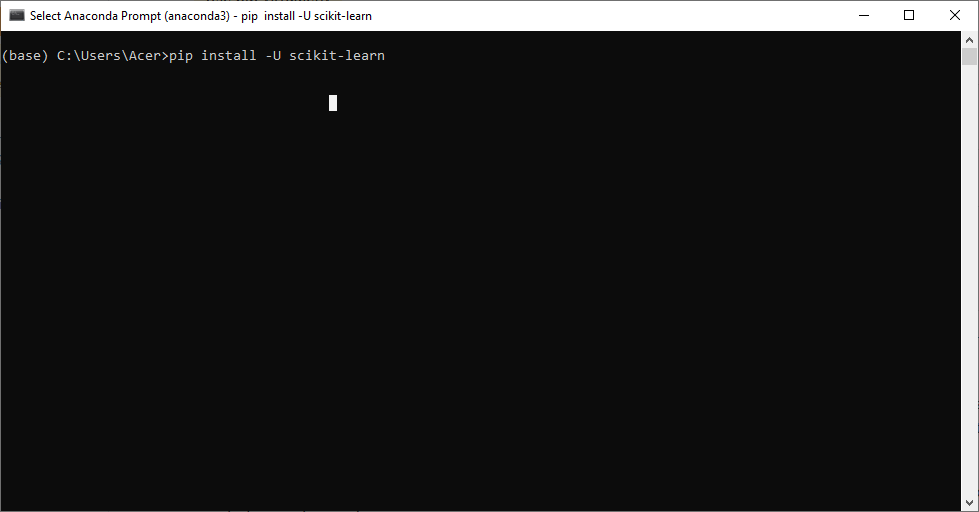
\includegraphics[scale=0.4]{figures/1.PNG}
		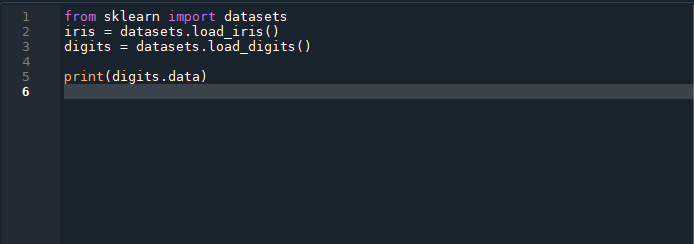
\includegraphics[scale=0.5]{figures/1a.PNG}
		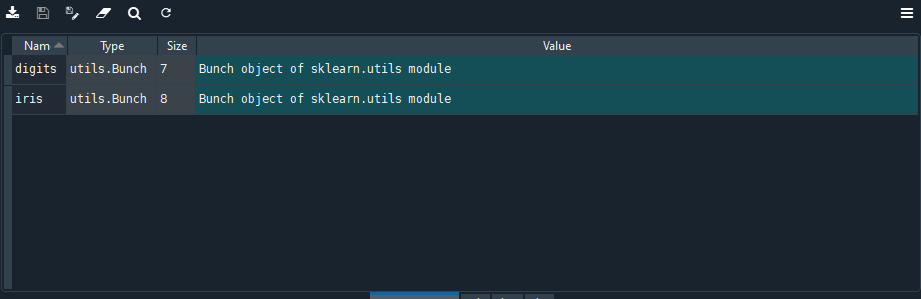
\includegraphics[scale=0.4]{figures/1b.PNG}
	\end{figure}

\newpage
\item
Mencoba Loading an example dataset, menjelaskan maksud dari tulisan tersebut dan mengartikan per baris.
	\begin{figure}[!htbp]
		\centering
		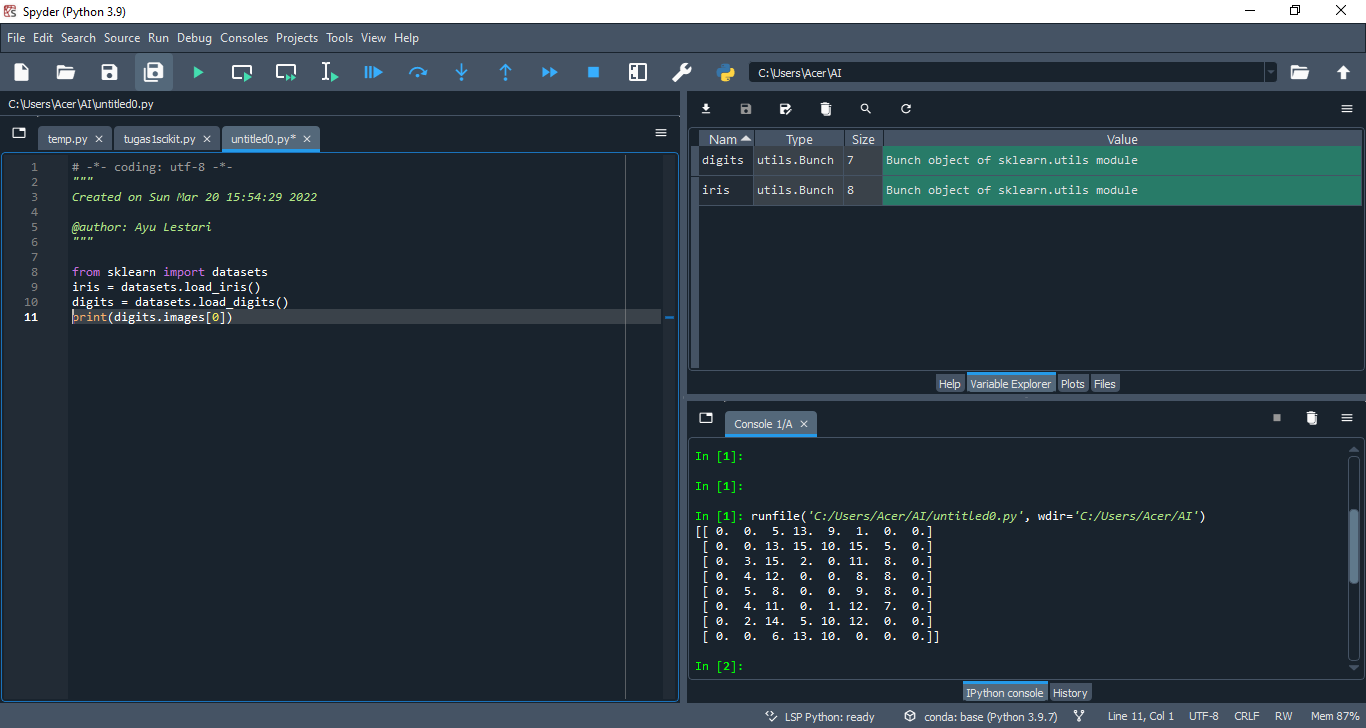
\includegraphics[scale=0.5]{figures/2.PNG}
		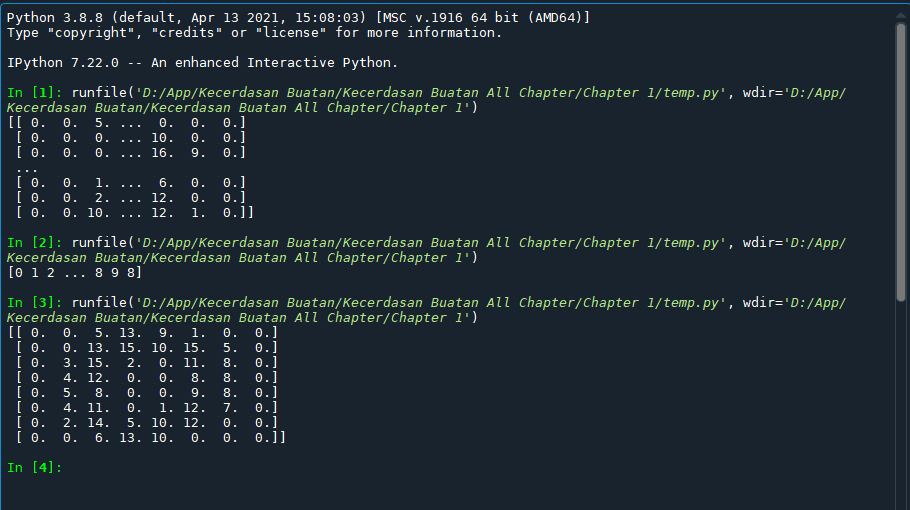
\includegraphics[scale=0.4]{figures/2a.PNG}
	\end{figure}

\newpage
\item
Mencoba Learning and predicting, menjelaskan maksud dari tulisan tersebut dan mengartikan per baris.
	\begin{figure}[!htbp]
		\centering
		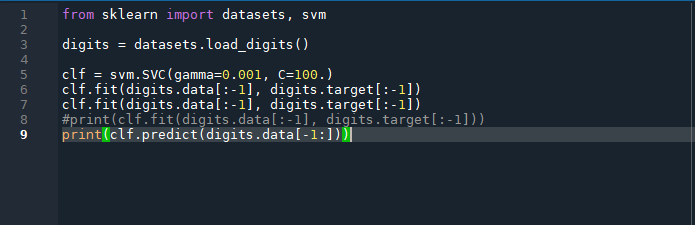
\includegraphics[scale=0.5]{figures/3.PNG}
		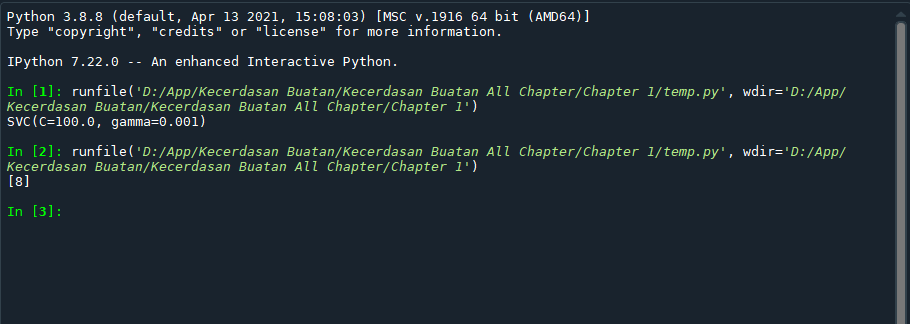
\includegraphics[scale=0.4]{figures/3a.PNG}
	\end{figure}


\item
Mencoba Model persistence, menjelaskan maksud dari tulisan tersebut dan mengartikan per baris. Terdapat dua cara yaitu menggunakan pickle atau menggunakan joblib.
	\begin{figure}[!htbp]
		\centering
		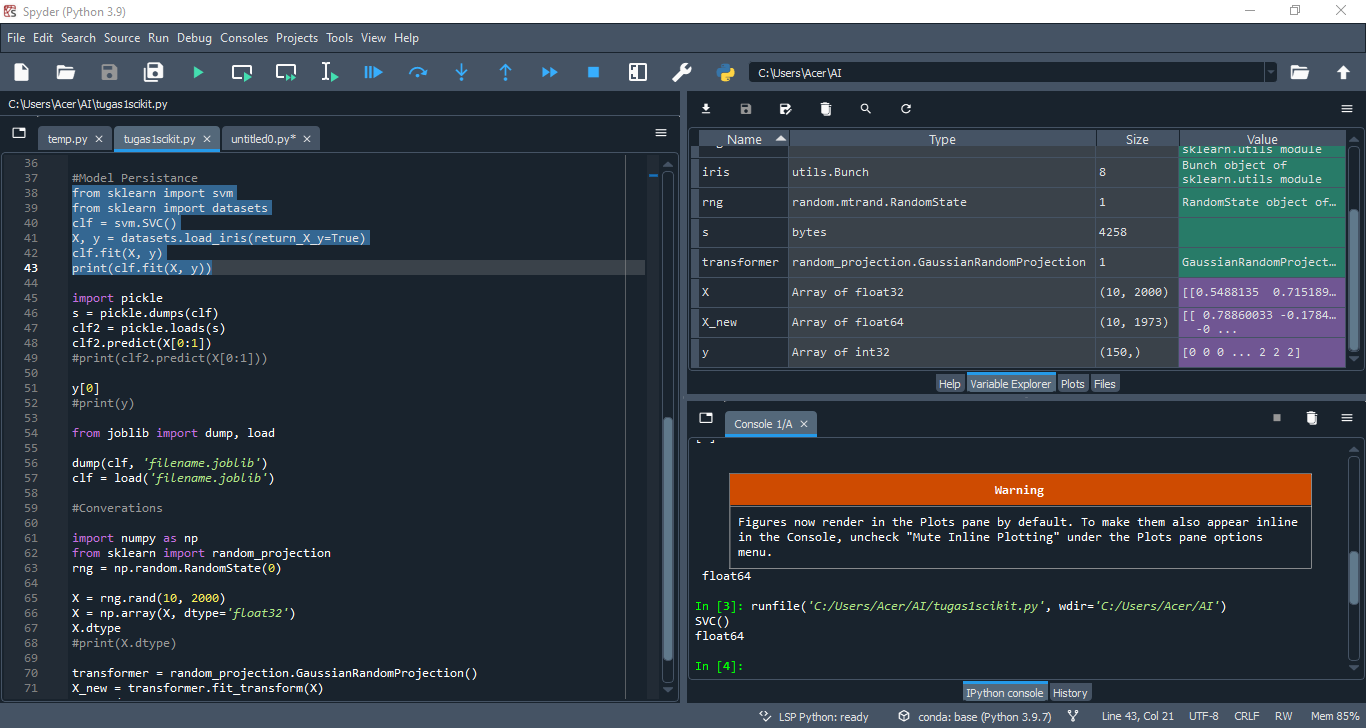
\includegraphics[scale=0.5]{figures/4.PNG}
		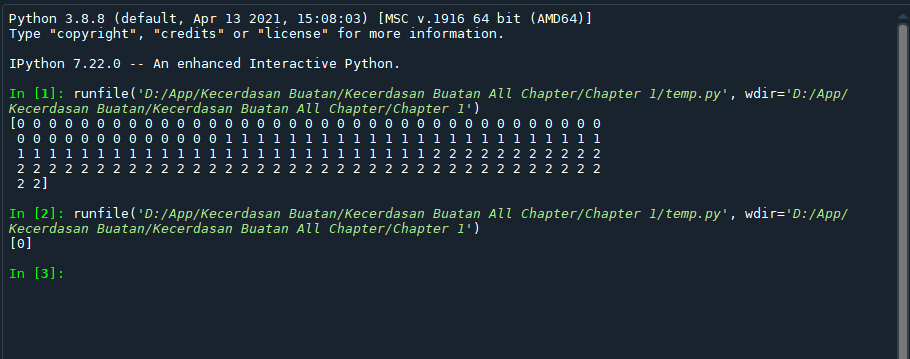
\includegraphics[scale=0.4]{figures/4a.PNG}
	\end{figure}

\newpage
\item 
Mencoba Conventions, menjelaskan maksud dari tulisan tersebut dan mengartikan per baris.
	\begin{figure}[!htbp]
		\centering
		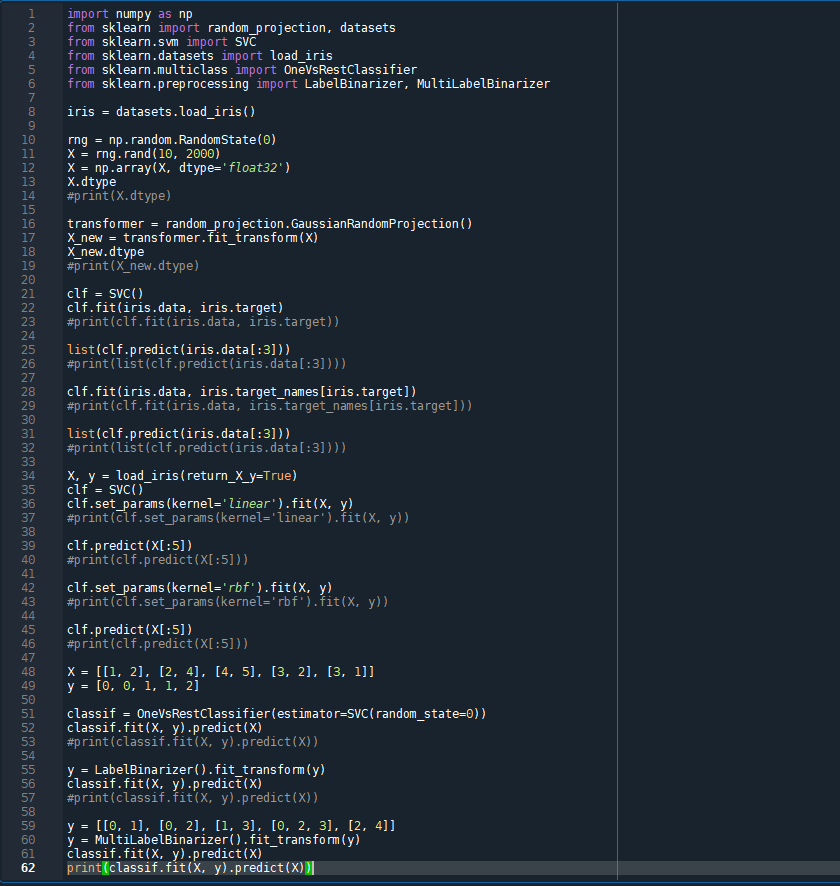
\includegraphics[scale=0.4]{figures/5.PNG}
		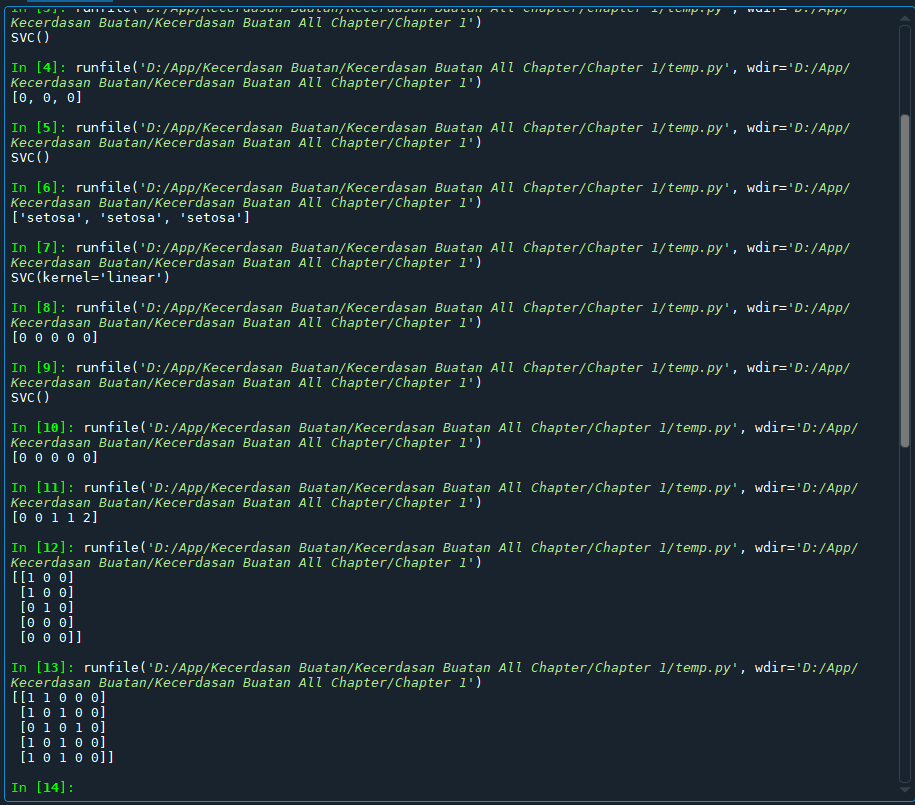
\includegraphics[scale=0.4]{figures/5a.PNG}
	\end{figure}

\end{enumerate}

\newpage
\section{Penanganan Error}
Dari percobaan yang dilakukan di atas, apabila mendapatkan error maka:

\begin{enumerate}
	\item Screenshot error.
	\begin{figure}[!htbp]
		\centering
		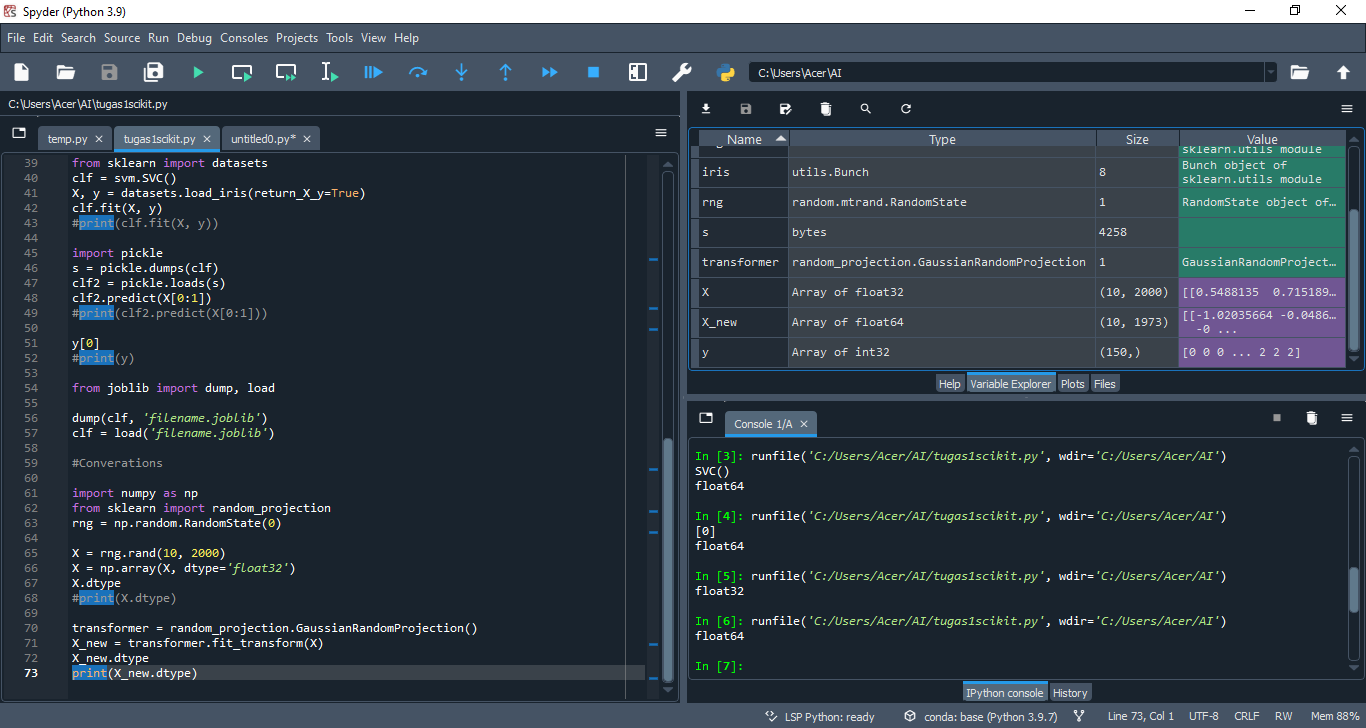
\includegraphics[scale=0.5]{figures/6.PNG}
		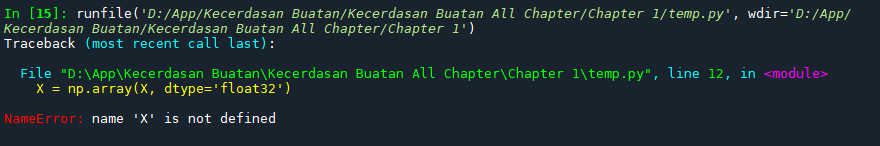
\includegraphics[scale=0.5]{figures/7.PNG}
	\end{figure}
	
	\item Tuliskan kode eror dan jenis errornya.
	\begin{enumerate}
		\item NotFittedError = This SVC instance is not fitted yet. Call ’fit’ with appropriate arguments before using this estimator.
		\item NameError = name ’X’ is not defined
	\end{enumerate}

	\item Solusi pemecahan masalah error tersebut.
	\begin{enumerate}
		\item NotFittedError = Solusinya yaitu memanggil parameter dengan method fit,
		sebelum menggunakan method predict.
		\item NameError = Solusinya yaitu membuat variabel dengan nama X.
	\end{enumerate}

\end{enumerate}


%\chapter{Membangun Model Prediksi}

\section{Teori}
Praktek teori penunjang yang dikerjakan(nilai 5 per nomor, untuk hari pertama) :
\begin{enumerate}
\item
Jelaskan apa itu binary classification dilengkapi ilustrasi gambar sendiri \\
\textit{Binary Classification} adalah mengklasifikasikan elemen - elemen himpunan menjadi 2 kelompok berdasarkan aturan klasifikasi.
\item
Jelaskan apa itu supervised learning dan unsupervised learning dan clustering dengan ilustrasi gambar sendiri. \\
\begin{itemize}
	\item Supervised Learning
	\par
		\textit{Supervised Learning} adalah suatu pendekatan machine learning yang ditentukan berdasarkan penggunaan dataset, supervised learning menggunakan dataset berlabel atau labeled dataset. Supervised Learning digunakan untuk melakukan klasifikasi data atau memprediksi hasil secara akurat sesuai dengan output berdasarkan pola yang ada didalam data training dan berupa data yang memiliki label yang sudah ditentukan terlebih dahulu. \\
		\begin{figure}[!htbp]
			\centering
			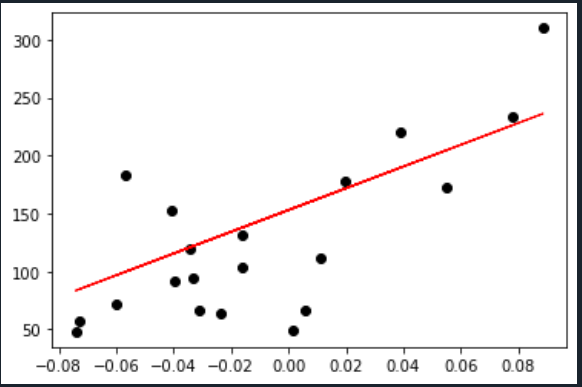
\includegraphics[scale=0.4]{figures/supervised-learning.PNG}
		\end{figure}
		\newpage
	\item Unsupervised Learning
	\par
		\textit{Unsupervised Learning} adalah pendekatan machine learning yang digunakan untuk menganalisa dan juga mengelompokan kumpulan - kumpulan data yang tidak berlabel.\\
		\begin{figure}[!htbp]
			\centering
			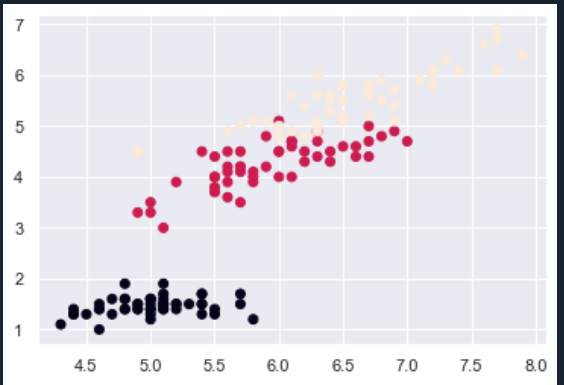
\includegraphics[scale=0.4]{figures/unsupervised-learning.PNG}
		\end{figure}
	\item Clustering
	\par
	\textit{Clustering} adalah sebuah proses pengelompokan data kedalam beberapa cluster sehingga data-data disuatu cluster memiliki kemiripan.\\
	\begin{figure}[!htbp]
		\centering
		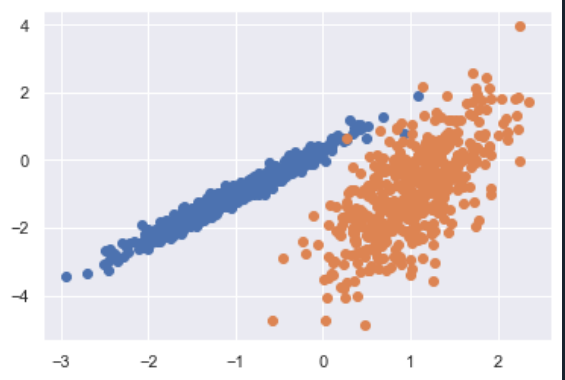
\includegraphics[scale=0.4]{figures/clustering.PNG}
	\end{figure}
	\par
	\item
	Jelaskan apa itu evaluasi dan akurasi dari buku dan disertai ilustrasi contoh dengan gambar sendiri
	\par
	\item 
	\textit{Evaluasi dan Akurasi}
	Evaluasi adalah bagaimana cara agar dapat mengevaluasi seberapa baiknya model bekerja dengan cara mengukur akurasinya.\\
	Akurasi memiliki definisi sebagai persentase kasus yang diklasifikasikan dengan benar.\\
	Kesalahan dari model dapat dianalisi menggunakan confusion matrix.\\
	\par
	\item
	Jelaskan bagaimana cara membuat dan membaca confusion matrix, buat confusion matrix buatan sendiri.
	\par
	\item 
	\textit{Confusion Matrix}\\ 
	1. Import dependencies yang dibutuhkan.\\
	2. Kemudian buat variabel untuk menampung value atau Nilai yang diprediksi.\\
	3. Buat variabel untuk menampung value atau nilai sebenarnya.\\
	4. Kemudian print confusion matrixnya dengan menggunakan variabel dari nilai sebenarnya dan variabel nilai yang diprediksi dengan label misalnya a,b,c.\\
	5. Kemudian print precision dan recall diantara matrix lainnya.
	\begin{figure}[!htbp]
		\centering
		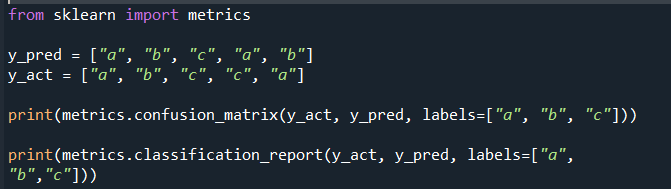
\includegraphics[scale=0.8]{figures/confusionmatrix.PNG}
	\end{figure}
	\begin{figure}[!htbp]
		\centering
		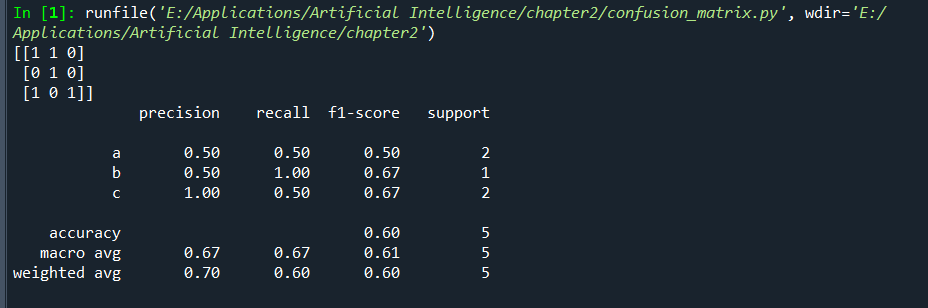
\includegraphics[scale=0.6]{figures/hasilconfusionmatrix.PNG}
	\end{figure}
	\item
	Jelaskan bagaimana K-fold cross validation bekerja dengan gambar ilustrasi contoh buatan sendiri.\\
	\item 
	1. Mengacak dataset secara random.\\
	2. Membagi dataset tersebut kedalam k-group, yaitu sebagai test dataset dan sisanya sebagai training dataset.\\
	3. Pasang model di set pelatihan dan evaluasi di set tes.\\
	4. Simpan skor evaluasi dan buang modelnya.\\
	5. Meringkas keterampilan model menggunakan sampel skor menggunakan model evaluasi.
	\item
	Jelaskan apa itu decision tree dengan gambar ilustrasi contoh buatan sendiri.
	\item 
	\textit{Decision Tree} adalah metode yang digunakan untuk membantu membuat keputusan dengan menggunakan model pohon untuk menampilkan keputusan, kemungkinan resiko, dan lainnya.
	\begin{figure}[!htbp]
		\centering
		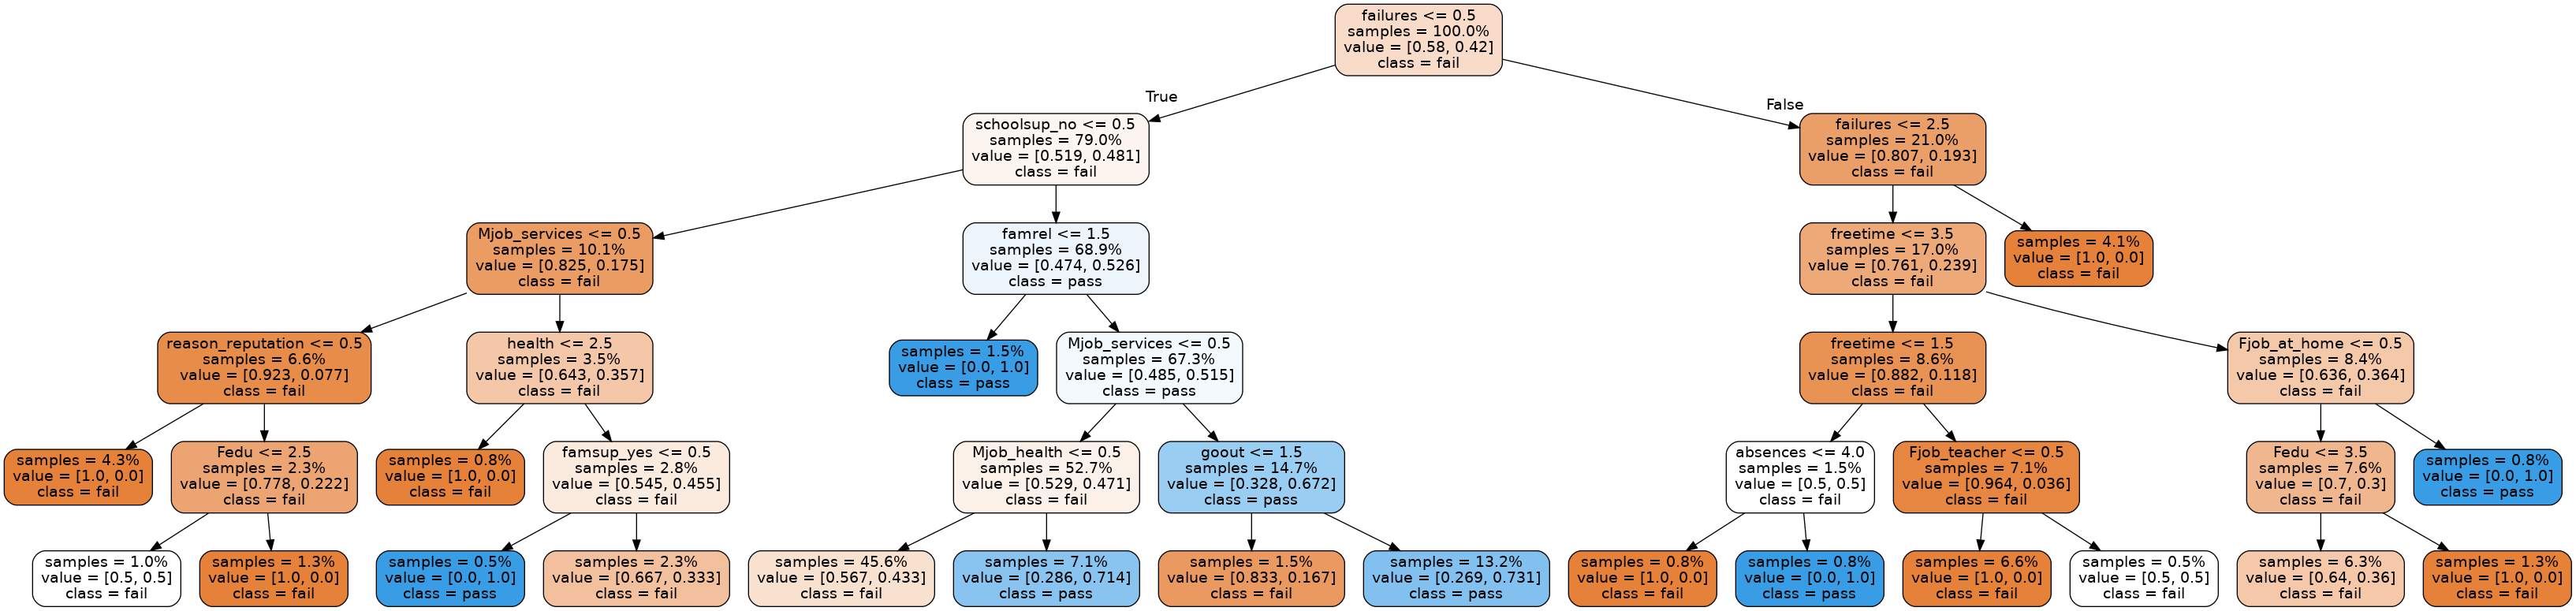
\includegraphics[scale=0.1]{figures/student-performance.PNG}
	\end{figure}
	\item
	Jelaskan apa itu information gain dan entropi dengan gambar ilustrasi buatan sendiri.
	\item 
	\textit{Information Gain} adalah sekumpulan informasi yang didapatkan dari variabel acak.\\
	\textit{Entropi} adalah tingkat keacakan dari informasi yang diperloh dari information gain yang sedang diproses.
\end{itemize}
\end{enumerate}

\section{scikit-learn}
Dataset ambil di https://github.com/PacktPublishing/Python-Artificial-Intelligence-Projects-for-Beginners folder Chapter01.
Tugas anda adalah, dataset ganti menggunakan \textbf{student-mat.csv} dan mengganti semua nama variabel dari kode di bawah ini dengan nama-nama makanan (NPM mod 3=0), kota (NPM mod 3=1), buah (NPM mod 3=2), . Jalankan satu per satu kode tersebut di spyder dengan menggunakan textit{Run current cell}. Kemudian Jelaskan dengan menggunakan bahasa yang mudah dimengerti dan bebas plagiat dan wajib skrinsut dari komputer sendiri masing masing nomor di bawah ini(nilai 5 masing masing pada hari kedua).

\begin{enumerate}

\item
\begin{verbatim}
	#1 Load dataset
	import pandas as pd
	apel = pd.read_csv('student-mat.csv', sep=';')
	len(apel)
\end{verbatim}
	Output :
\begin{figure}[!htbp]
	\centering
	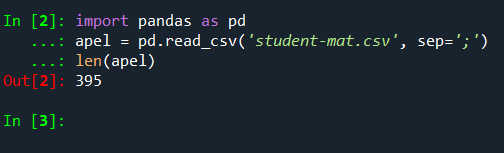
\includegraphics[scale=0.8]{figures/loaddataset1.PNG}
\end{figure}
\item
\begin{verbatim}
	#2 generate binary label (pass)
	# (test grades, each 0-20 pts); threshold for passing is sum>=30
	
	apel['pass'] = apel.apply(lambda row: 1 if (row['G1']+row['G2']+row['G3']) >= 35 else 0, axis=1)
	apel = apel.drop(['G1', 'G2', 'G3'], axis=1)
	apel.head()
\end{verbatim}
	Output :
\begin{figure}[!htbp]
	\centering
	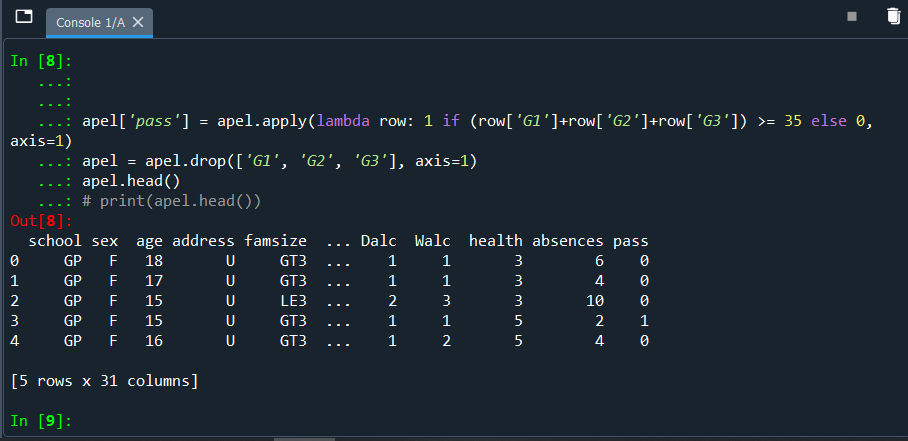
\includegraphics[scale=0.8]{figures/generate_binarylabel.PNG}
\end{figure}
\newpage
\item
\begin{verbatim}
	# 3 use one-hot encoding on categorical columns
	apel = pd.get_dummies(apel, columns=['sex', 'school', 'address', 'famsize', 'Pstatus', 'Mjob', 'Fjob', 
	'reason', 'guardian', 'schoolsup', 'famsup', 'paid', 'activities',
	'nursery', 'higher', 'internet', 'romantic'])
	apel.head()
\end{verbatim}
	Output :
\begin{figure}[!htbp]
	\centering
	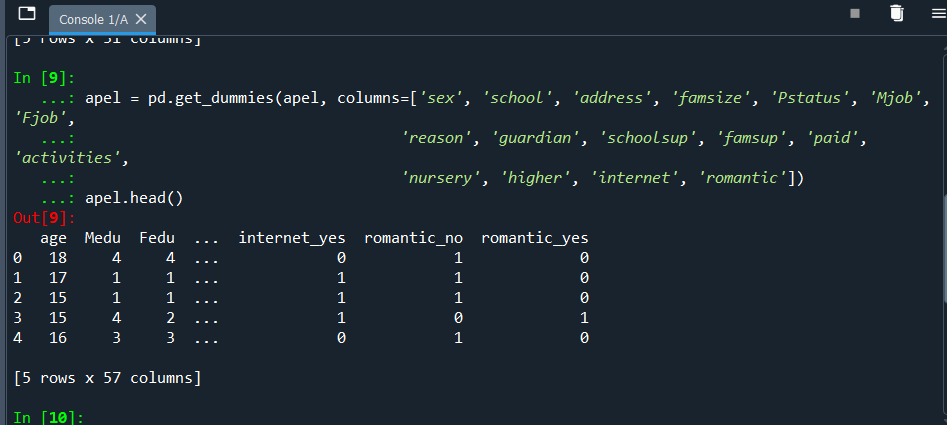
\includegraphics[scale=0.8]{figures/encodingoncategoricalcolumns.PNG}
\end{figure}
\item
\begin{verbatim}
# 4 shuffle rows
apel = apel.sample(frac=1)
#   split traning and testing data
apel_train = apel[:500]
apel_test = apel[:500]

apel_train_att = apel_train.drop(['pass'], axis=1)
apel_train_pass = apel_train['pass']

apel_test_att = apel_test.drop(['pass'], axis=1)
apel_test_pass = apel_test['pass']

apel_att = apel.drop(['pass'], axis=1)
apel_pass = apel['pass']

# number off passing students in whole dataset:
import numpy as np
print("Passing: %d out of %d (%.2f%%)" % (np.sum(apel_pass), len(apel_pass), 
100*float(np.sum(apel_pass)) / len(apel_pass)))
\end{verbatim}
	Output :
\begin{figure}[!htbp]
	\centering
	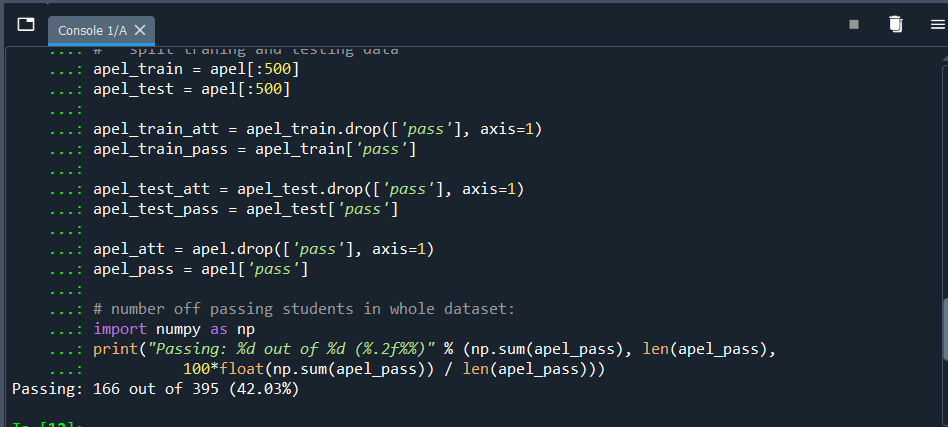
\includegraphics[scale=0.8]{figures/shufflerows.PNG}
\end{figure}
\item 
\begin{verbatim}
	# 5 fit a decision tree
	from sklearn import tree
	semangka = tree.DecisionTreeClassifier(criterion="entropy", max_depth=5)
	semangka = semangka.fit(apel_train_att, apel_train_pass)
\end{verbatim}
\begin{figure}[!htbp]
	\centering
	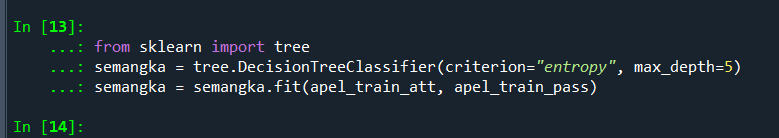
\includegraphics[scale=0.8]{figures/fitdecisontree.PNG}
\end{figure}
\item
\begin{verbatim}
	# 6 visualize tree
	import graphviz
	dot_data = tree.export_graphviz(semangka, out_file=None, label="all", 
	impurity=False, proportion=True,
	feature_names=list(apel_train_att), 
	class_names=["fail", "pass"], 
	filled=True, rounded=True)
	graph = graphviz.Source(dot_data)
	graph
\end{verbatim}
\begin{figure}[!htbp]
	\centering
	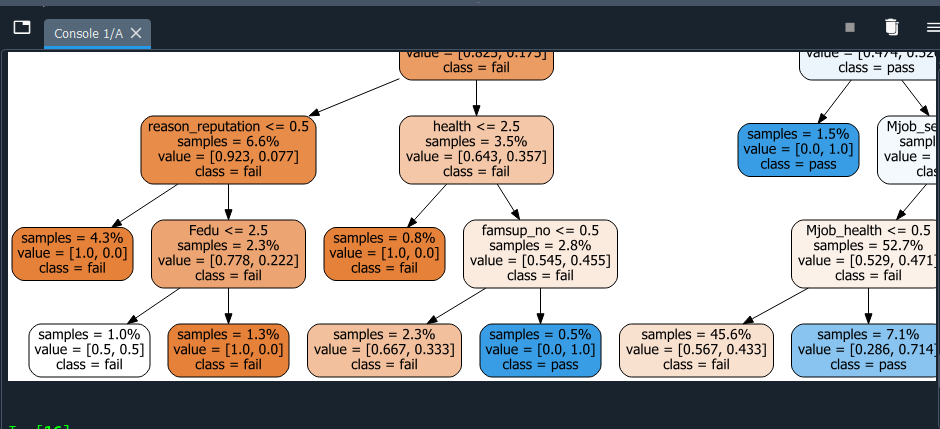
\includegraphics[scale=0.8]{figures/visualizetree.PNG}
\end{figure}
\item
\begin{verbatim}
	# 7 save tree
	tree.export_graphviz(semangka, out_file="student-performance.dot", 
	label="all", impurity=False, 
	proportion=True,
	feature_names=list(apel_train_att), 
	class_names=["fail", "pass"], 
	filled=True, rounded=True)
\end{verbatim}
\begin{figure}[!htbp]
	\centering
	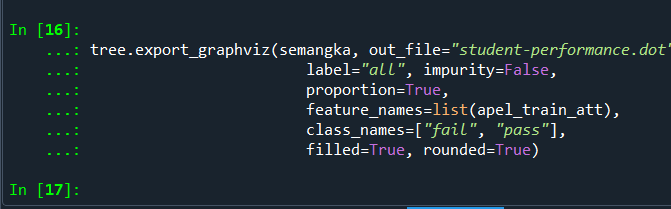
\includegraphics[scale=0.8]{figures/savetree.PNG}
\end{figure}
\item
\begin{verbatim}
	# 8
	semangka.score(apel_test_att, apel_test_pass)
\end{verbatim}
\begin{figure}[!htbp]
	\centering
	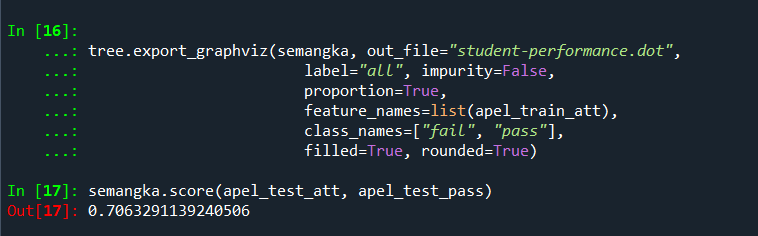
\includegraphics[scale=0.8]{figures/8.PNG}
\end{figure}
\item
\begin{verbatim}
	# 9
	from sklearn.model_selection import cross_val_score
	salak = cross_val_score(semangka, apel_att, apel_pass, cv=5)
	# show average score and +/- two standard deviations away 
	#(covering 95% of scores)
	print("Accuracy: %0.2f (+/- %0.2f)" % (salak.mean(), salak.std() * 2))
\end{verbatim}
\begin{figure}[!htbp]
	\centering
	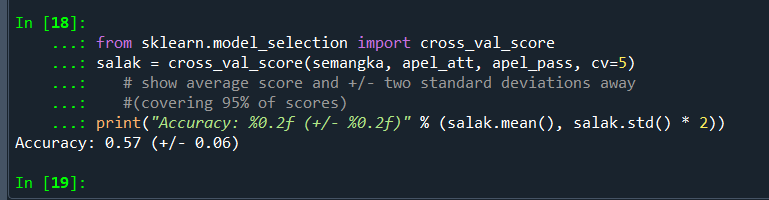
\includegraphics[scale=0.8]{figures/9.PNG}
\end{figure}
\item 
\begin{verbatim}
	# 10
	for max_depth in range(1, 20):
	semangka = tree.DecisionTreeClassifier(criterion="entropy", 
	max_depth=max_depth)
	salak = cross_val_score(semangka, apel_att, apel_pass, cv=5)
	print("Max depth: %d, Accuracy: %0.2f (+/- %0.2f)" % 
	(max_depth, salak.mean(), salak.std() * 2)
	)
\end{verbatim}
\begin{figure}[!htbp]
	\centering
	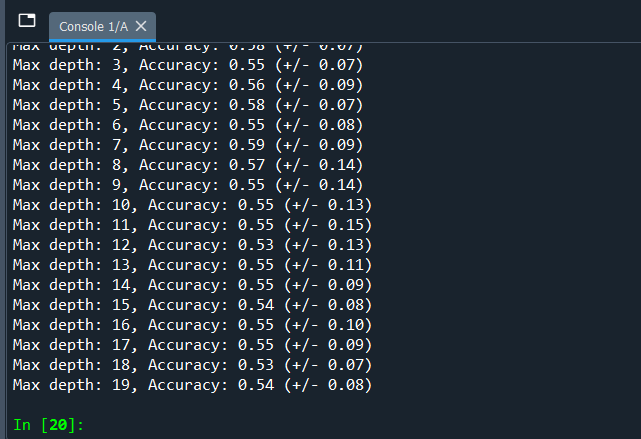
\includegraphics[scale=0.8]{figures/10.PNG}
\end{figure}
\newpage
\item
\begin{verbatim}
	# 11
	depth_acc = np.empty((19,3), float)
	i = 0
	for max_depth in range(1, 20):
	semangka = tree.DecisionTreeClassifier(criterion="entropy", 
	max_depth=max_depth)
	salak = cross_val_score(semangka, apel_att, apel_pass, cv=5)
	depth_acc[i,0] = max_depth
	depth_acc[i,1] = salak.mean()
	depth_acc[i,2] = salak.std() * 2
	i += 1
	depth_acc
\end{verbatim}
\begin{figure}[!htbp]
	\centering
	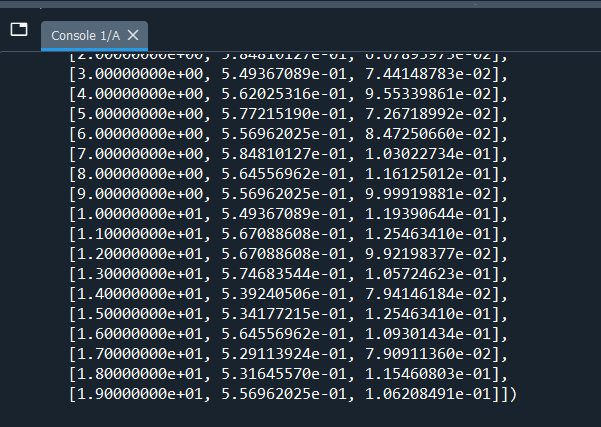
\includegraphics[scale=0.8]{figures/11.PNG}
\end{figure}
\item 
\begin{verbatim}
	# 12
	import matplotlib.pyplot as plt
	fig, ax = plt.subplots()
	ax.errorbar(depth_acc[:,0], depth_acc[:,1], yerr=depth_acc[:,2])
	plt.show()
\end{verbatim}
\begin{figure}[!htbp]
	\centering
	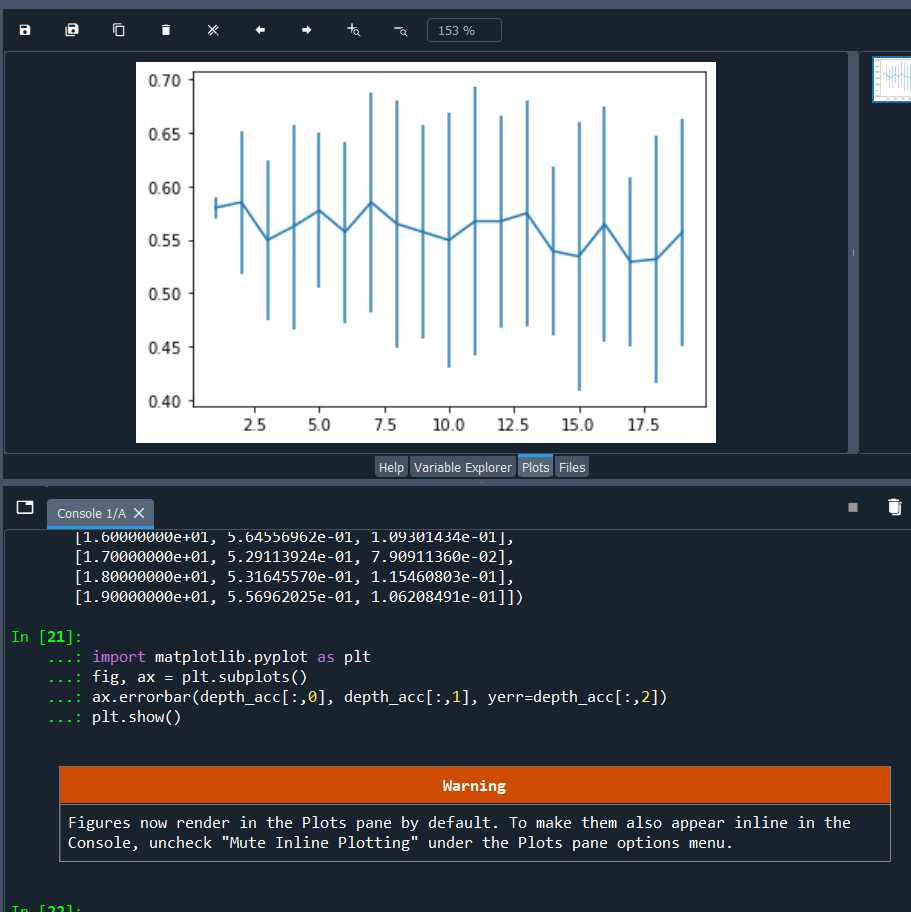
\includegraphics[scale=0.6]{figures/12.PNG}
\end{figure}
\newpage

\end{enumerate}
Link Youtube : https://youtu.be/2aM5RLBPp1c

\section{Penanganan Error}
Dari percobaan yang dilakukan di atas, error yang kita dapatkan di dokumentasikan dan di selesaikan(nilai 5 hari kedua):

\begin{enumerate}
	\item
skrinsut error
\begin{figure}[!htbp]
	\centering
	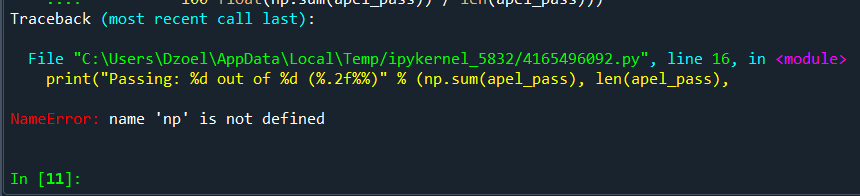
\includegraphics[scale=0.8]{figures/np_not_defined_error.PNG}
\end{figure}
	\item
Tuliskan kode eror dan jenis errornya\\
NameError : name 'np' is not defined
	\item
Solusi pemecahan masalah error tersebut\\
Solusinya adalah import numpy dengan alias np.

\end{enumerate}


%\chapter{Prediksi dengan Random Forest}

Untuk pratikum saati ini menggunakan buku \textit{Python Artificial Intelligence Projects for Beginners}\cite{eckroth2018python}. Dengan praktek menggunakan python 3 dan editor anaconda dan library python scikit-learn.
Kode program ada di https://github.com/PacktPublishing/Python-Artificial-Intelligence-Projects-for-Beginners .
Tujuan pembelajaran pada pertemuan pertama antara lain:
\begin{enumerate}
    \item
          Mengerti implementasi klasifikasi dan teknik evaluasi
    \item
          Memprediksi spesies burung dengan random forest
    \item
          Memahami Confusion Matrix.
\end{enumerate}
Tugas dengan cara dikumpulkan dengan pull request ke github dengan menggunakan latex pada repo yang dibuat oleh asisten riset. Kode program menggunakan input listing ditaruh di folder src ekstensi .py dan dipanggil ke latex dengan input listings. Tulisan dan kode tidak boleh plagiat, menggunakan bahasa indonesia yang sesuai dengan gaya bahasa buku teks.

\section{Teori}
Random Forest adalah hasil voting dari beberapa decission tree yang masing-masing memegang atribut yang berbeda. Jadi setiap decission tree spesifik terhadap atribut tersebut yang merupakan bagian kecil dari keseluruhan atribut di data set. Hindari RF jika atribut terlalu sedikit untuk membentuk beberapa tree. Pada praktek kali ini mengggunakan dataset spesies burung yang diambil dari situs
(http://www.vision.caltech.edu/visipedia/CUB-200-2011.html). Didalamnya terdapat 12.000 foto dari 200 spesies yang berbeda. Yang akan kita pakai untuk RF hanya atribut dari burunynya saja seperti ukuran, bentuk dan warna. Data tersebut diberi label secara manual oleh manusia dengan memanfaatkan jasa dari Amazon's Mechanical Turk.

\subsection{Random Forest}
Pertama dataset kita baca terlebih dahulu.
\begin{lstlisting}[caption=Membaca data file txt,label={lst:fungsisederhana}]
import pandas as pd

# some lines have too many fields (?), so skip bad lines
imgatt = pd.read_csv("data/CUB_200_2011/attributes/image_attribute_labels.txt",
                     sep='\s+', header=None, error_bad_lines=False, warn_bad_lines=False,
                     usecols=[0,1,2], names=['imgid', 'attid', 'present'])

\end{lstlisting}

Melihat sebagian data awal, dengan menggunakan listing \ref{lst:3.1}.

\begin{lstlisting}[caption=Melihat sebagian data awal,label={lst:3.1}]
imgatt.head()
\end{lstlisting}

Melihat jumlah data menggunakan listing \ref{lst:3.2}.
\begin{lstlisting}[caption=Mengetahui jumlah data,label={lst:3.2}]
imgatt.shape
\end{lstlisting}

Merubah atribut menjadi kolom dengan menggunakan pivot layaknya excel. lalu kita cek isinya dengan menggunakan perintah pada listing \ref{lst:3.3}.
\begin{lstlisting}[caption=Pivot dataset,label={lst:3.3}]
imgatt2 = imgatt.pivot(index='imgid', columns='attid', values='present')

imgatt2.head()
imgatt2.shape
\end{lstlisting}


Sekarang kita akan meload jawabannya yang berisi apakah burung itu termasuk dalam spesies yang mana. Dua kolomnya adalah imgid dan label. Dan melakukan pivot yang mana imgid menjadi index yang artinya unik perintahnya ada di listing \ref{lst:3.6}. Lalu kita cek kembali datanya.
\begin{lstlisting}[caption=membaca dataset label file txt,label={lst:3.6}]
imglabels = pd.read_csv("data/CUB_200_2011/image_class_labels.txt", 
                        sep=' ', header=None, names=['imgid', 'label'])

imglabels = imglabels.set_index('imgid')


imglabels.head()
imglabels.shape
\end{lstlisting}

Karena isinya sama kita bisa melakukan join antara dua data. Sehingga kita akan mendapatkan data ciri dan data jawabannya atau labelnya sehingga bisa dikatekorikan supervised learning. maka perintah untuk menggabungkan kedua data dan kemudian kita melakukan pemisahan antara data set untuk training dan test dengan perintah di listing \ref{lst:3.7}.
\begin{lstlisting}[caption=Menggabungkan field dari dua file terpisah,label={lst:3.7}]
df = imgatt2.join(imglabels)
df = df.sample(frac=1)
\end{lstlisting}

Kemudian drop label yang didepan, dan gunakan label yang paling belakang yang baru di join dengan perintah listing \ref{lst:3.8}.
\begin{lstlisting}[caption=Memisahkan dan memilih label,label={lst:3.8}]
df_att = df.iloc[:, :312]
df_label = df.iloc[:, 312:]
\end{lstlisting}
Kita bisa mengecek isinya dengan perintah listing \ref{lst:3.9}.
\begin{lstlisting}[caption=Melihat isi masing masing data frame,label={lst:3.9}]
df_att.head()
df_label.head()
\end{lstlisting}

Kita bagi menjadi dua bagian, 8000 row pertama sebagai data training sisanya sebagai data testing dengan perintah listing \ref{lst:3.10}.
\begin{lstlisting}[caption=Pembagian data training dan test,label={lst:3.10}]
df_train_att = df_att[:8000]
df_train_label = df_label[:8000]
df_test_att = df_att[8000:]
df_test_label = df_label[8000:]

df_train_label = df_train_label['label']
df_test_label = df_test_label['label']
\end{lstlisting}

Kita panggil kelas RandomForestClassifier. max features diartikan sebagai berapa banyak kolom pada setiap tree dengan perintah listing \ref{lst:3.11}.
\begin{lstlisting}[caption=Instansiasi kelas Random Forest,label={lst:3.11}]
from sklearn.ensemble import RandomForestClassifier
clf = RandomForestClassifier(max_features=50, random_state=0, n_estimators=100)

\end{lstlisting}
Kemudian lakukan fit untuk membangun random forest yang sudah ditentukan dengan maksimum fitur sebanya 50 untuk perpohonnya dengan perintah listing \ref{lst:3.12}.

\begin{lstlisting}[caption=Fitting random forest dengan dataset training,label={lst:3.12}]
clf.fit(df_train_att, df_train_label)
\end{lstlisting}
Hasilnya bisa kita dapatkan dengan perintah predict dengan perintah listing \ref{lst:3.13}.
\begin{lstlisting}[caption=Melihat Hasil prediksi,label={lst:3.13}]
print(clf.predict(df_train_att.head()))
\end{lstlisting}

Untuk besaran akurasinya dengan perintah listing \ref{lst:3.14}
\begin{lstlisting}[caption=Score perolehan dari klasifikasi,label={lst:3.14}]
clf.score(df_test_att, df_test_label)
\end{lstlisting}

\subsection{Confusion Matrix}
Dari RF kita coba petakan ke dalam Confusion Matrix dan lihat hasilnya dengan perintah listing \ref{lst:3.15}.
\begin{lstlisting}[caption=Membuat Confusion Matrix,label={lst:3.15}]
from sklearn.metrics import confusion_matrix
pred_labels = clf.predict(df_test_att)
cm = confusion_matrix(df_test_label, pred_labels)

cm
\end{lstlisting}

Kemudian kita plot dengan perintah
\begin{lstlisting}[caption=Plotting Confusion Matrix,label={lst:3.16}]
import matplotlib.pyplot as plt
import itertools
def plot_confusion_matrix(cm, classes,
                          normalize=False,
                          title='Confusion matrix',
                          cmap=plt.cm.Blues):
    """
    This function prints and plots the confusion matrix.
    Normalization can be applied by setting `normalize=True`.
    """
    if normalize:
        cm = cm.astype('float') / cm.sum(axis=1)[:, np.newaxis]
        print("Normalized confusion matrix")
    else:
        print('Confusion matrix, without normalization')

    print(cm)

    plt.imshow(cm, interpolation='nearest', cmap=cmap)
    plt.title(title)
    #plt.colorbar()
    tick_marks = np.arange(len(classes))
    plt.xticks(tick_marks, classes, rotation=90)
    plt.yticks(tick_marks, classes)

    fmt = '.2f' if normalize else 'd'
    thresh = cm.max() / 2.
    #for i, j in itertools.product(range(cm.shape[0]), range(cm.shape[1])):
    #    plt.text(j, i, format(cm[i, j], fmt),
    #             horizontalalignment="center",
    #             color="white" if cm[i, j] > thresh else "black")

    plt.tight_layout()
    plt.ylabel('True label')
    plt.xlabel('Predicted label')

\end{lstlisting}

Agar plot sumbunya sesuai dengan nama datanya maka kita set dengan perintah
\begin{lstlisting}[caption=Membaca file classes.txt,label={lst:3.17}]
birds = pd.read_csv("data/CUB_200_2011/classes.txt",
                    sep='\s+', header=None, usecols=[1], names=['birdname'])
birds = birds['birdname']
birds

\end{lstlisting}

Lalu kita plot
\begin{lstlisting}[caption=Plot hasil perubahan label,label={lst:3.18}]
import numpy as np
np.set_printoptions(precision=2)
plt.figure(figsize=(60,60), dpi=300)
plot_confusion_matrix(cm, classes=birds, normalize=True)
plt.show()
\end{lstlisting}



\subsection{Mencoba dengan metode Decission Tree dan SVM}
Kita coba menggunakan Decission tree
\begin{lstlisting}[caption=Mencoba klasifikasi dengan decission tree dengan dataset yang sama,label={lst:3.19}]
from sklearn import tree
clftree = tree.DecisionTreeClassifier()
clftree.fit(df_train_att, df_train_label)
clftree.score(df_test_att, df_test_label)
\end{lstlisting}
Kita coba menggunakan SVM
\begin{lstlisting}[caption=Mencoba klasifikasi dengan SVM dengan dataset yang sama,label={lst:3.20}]
from sklearn import svm
clfsvm = svm.SVC()
clfsvm.fit(df_train_att, df_train_label)
clfsvm.score(df_test_att, df_test_label)
\end{lstlisting}

\subsection{Pengecekan Cross Validation}
Pengeceken Cross Validation untuk random forest
\begin{lstlisting}[caption=Hasil Cross Validation random forest,label={lst:3.21}]
from sklearn.model_selection import cross_val_score
scores = cross_val_score(clf, df_train_att, df_train_label, cv=5)
# show average score and +/- two standard deviations away (covering 95% of scores)
print("Accuracy: %0.2f (+/- %0.2f)" % (scores.mean(), scores.std() * 2))
\end{lstlisting}
untuk decission tree
\begin{lstlisting}[caption=Hasil Cross Validation Decission Tree,label={lst:3.22}]
scorestree = cross_val_score(clftree, df_train_att, df_train_label, cv=5)
print("Accuracy: %0.2f (+/- %0.2f)" % (scorestree.mean(), scorestree.std() * 2))
\end{lstlisting}
untuk SVM
\begin{lstlisting}[caption=Hasil Cross Validation SVM,label={lst:3.23}]
scoressvm = cross_val_score(clfsvm, df_train_att, df_train_label, cv=5)
print("Accuracy: %0.2f (+/- %0.2f)" % (scoressvm.mean(), scoressvm.std() * 2))
\end{lstlisting}



\subsection{Pengamatan komponen informasi}
Untuk mengetahui berapa banyak tree yang dibuat, berapa banyak atribut yang dipakai dan informasi lainnya menggunakan kode
\begin{lstlisting}[caption=Melakukan Pengamatan komponen informasi,label={lst:3.24}]
max_features_opts = range(5, 50, 5)
n_estimators_opts = range(10, 200, 20)
rf_params = np.empty((len(max_features_opts)*len(n_estimators_opts),4), float)
i = 0
for max_features in max_features_opts:
    for n_estimators in n_estimators_opts:
        clf = RandomForestClassifier(max_features=max_features, n_estimators=n_estimators)
        scores = cross_val_score(clf, df_train_att, df_train_label, cv=5)
        rf_params[i,0] = max_features
        rf_params[i,1] = n_estimators
        rf_params[i,2] = scores.mean()
        rf_params[i,3] = scores.std() * 2
        i += 1
        print("Max features: %d, num estimators: %d, accuracy: %0.2f (+/- %0.2f)" %               (max_features, n_estimators, scores.mean(), scores.std() * 2))

\end{lstlisting}
Dan kita bisa melakukan plot informasi ini dengan kode
\begin{lstlisting}[caption=Plot Komponen informasi agar bisa dibaca,label={lst:3.25}]
import matplotlib.pyplot as plt
from mpl_toolkits.mplot3d import Axes3D
from matplotlib import cm
fig = plt.figure()
fig.clf()
ax = fig.gca(projection='3d')
x = rf_params[:,0]
y = rf_params[:,1]
z = rf_params[:,2]
ax.scatter(x, y, z)
ax.set_zlim(0.2, 0.5)
ax.set_xlabel('Max features')
ax.set_ylabel('Num estimators')
ax.set_zlabel('Avg accuracy')
plt.show()
\end{lstlisting}




\section{Soal Teori}
Praktek teori penunjang yang dikerjakan(nilai 5 per nomor, untuk hari pertama) :
\begin{enumerate}
    \item
          Jelaskan apa itu random forest, sertakan gambar ilustrasi buatan sendiri.
    \item
          Jelaskan cara membaca dataset kasus dan artikan makna setiap file dan isi field masing masing file.
    \item
          Jelaskan apa itu cross validation
    \item
          Jelaskan apa arti score 44\% pada random forest, 27\% pada decission tree dan 29\%dari SVM.
    \item
          Jelaskan bagaimana cara membaca confusion matriks dan contohnya memakai gambar atau ilustrasi sendiri.
    \item
          Jelaskan apa itu voting pada random forest disertai dengan ilustrasi gambar sendiri.
\end{enumerate}

\section{Praktek Program}
Tugas anda adalah,praktekkan dan jelaskan dengan menggunakan bahasa yang mudah dimengerti dan bebas plagiat dan wajib skrinsut dari komputer sendiri masing masing nomor di bawah ini(nilai 5 masing masing pada hari kedua).

\begin{enumerate}
    \item buat aplikasi sederhana menggunakan pandas dan jelaskan arti setiap baris kode yang dibuat(harus beda dengan teman sekelas)
          \begin{figure}[ht]
              \centerline{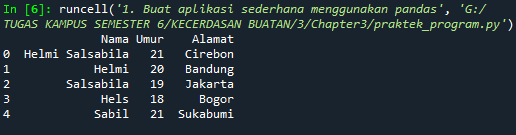
\includegraphics[scale=0.7]{figures/chapter3-1.png}}
              \caption{Aplikasi Pandas - Chapter3}
              \label{Aplikasi Pandas - Chapter3}
          \end{figure}

    \item buat aplikasi sederhana menggunakan numpy dan jelaskan arti dari setiap baris kode yang dibuat(harus beda dengan teman sekelas)
          \begin{figure}[ht]
              \centerline{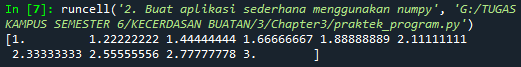
\includegraphics[scale=0.7]{figures/chapter3-2.png}}
              \caption{Aplikasi Numpy - Chapter3}
              \label{Aplikasi Numpy - Chapter3}
          \end{figure}

    \item buat aplikasi sederhana menggunakan matplotlib dan jelaskan arti dari setiap baris kode(harus beda dengan teman sekelas)
          \begin{figure}[ht]
              \centerline{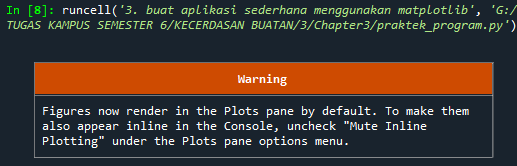
\includegraphics[scale=0.7]{figures/chapter3-3.png}}
              \centerline{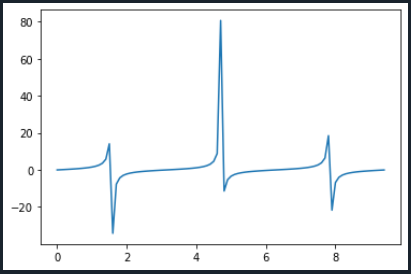
\includegraphics[scale=0.7]{figures/chapter3-3a.png}}
              \caption{Aplikasi Matplotlib - Chapter3}
              \label{Aplikasi Matplotlib - Chapter3}
          \end{figure}

    \item jalankan program klasifikasi Random Fores pada bagian teori bab ini. Tunjukkan keluarannya dari komputer sendiri dan artikan maksud setiap luaran yang didapatkan.
          \begin{figure}[ht]
              \centerline{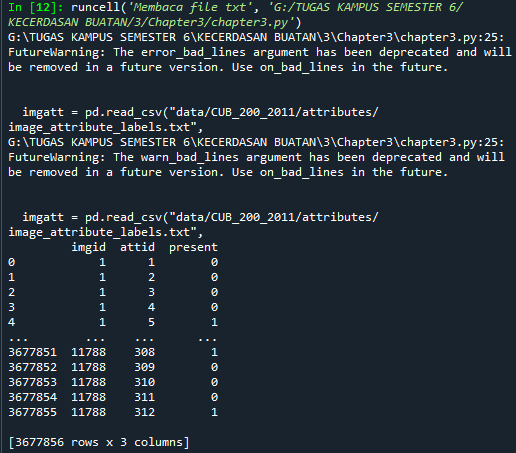
\includegraphics[scale=0.7]{figures/chapter3-4.png}}
              \centerline{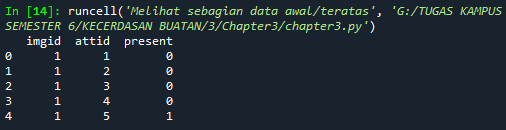
\includegraphics[scale=0.7]{figures/chapter3-4a.png}}
              \centerline{
\includegraphics[scale=0.7]{figures/chapter3-4b.png}}
              \centerline{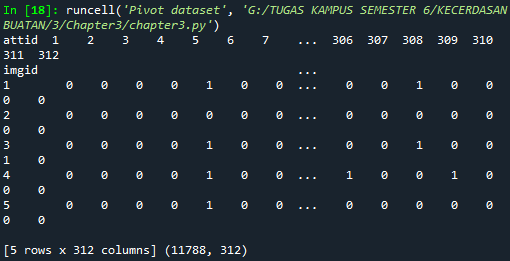
\includegraphics[scale=0.7]{figures/chapter3-4c.png}}
          \end{figure}
          \newpage
          \begin{figure}[ht]
              \centerline{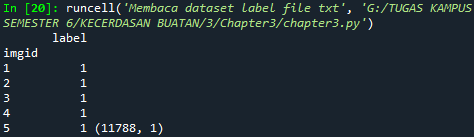
\includegraphics[scale=0.7]{figures/chapter3-4d.png}}
              \centerline{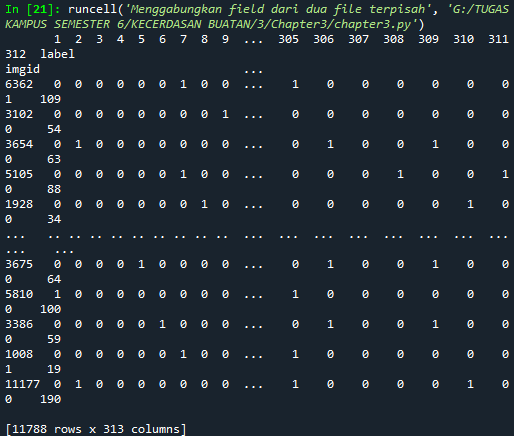
\includegraphics[scale=0.7]{figures/chapter3-4e.png}}
          \end{figure}
          \newpage
          \begin{figure}[ht]
              \centerline{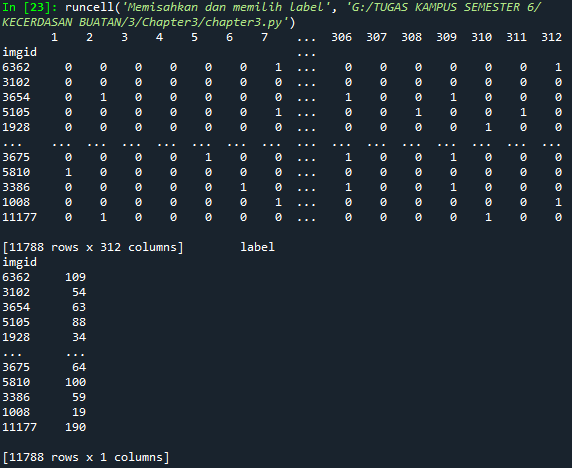
\includegraphics[scale=0.7]{figures/chapter3-4f.png}}
              \centerline{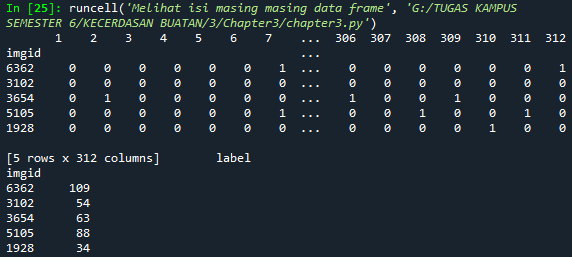
\includegraphics[scale=0.7]{figures/chapter3-4g.png}}
          \end{figure}
          \newpage
          \begin{figure}[ht]
              \centerline{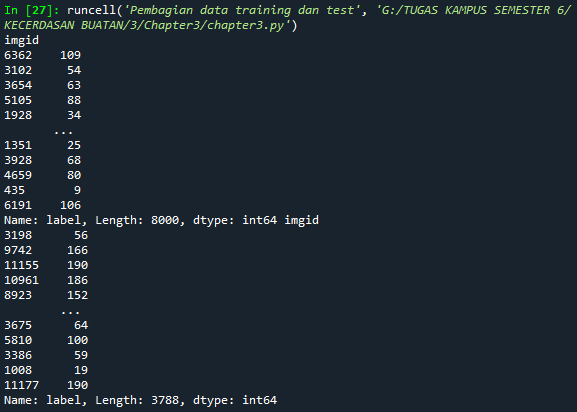
\includegraphics[scale=0.7]{figures/chapter3-4h.png}}
              \centerline{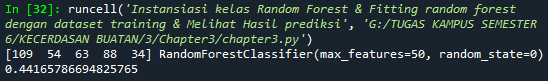
\includegraphics[scale=0.7]{figures/chapter3-4i.png}}
              \caption{Klasifikasi Random Fores - Chapter3}
              \label{Klasifikasi Random Fores - Chapter3}
          \end{figure}
          \newpage

    \item jalankan program confusion matrix pada bagian teori bab ini. Tunjukkan keluarannya dari komputer sendiri dan artikan maksud setiap luaran yang didapatkan.
          \begin{figure}[ht]
              \centerline{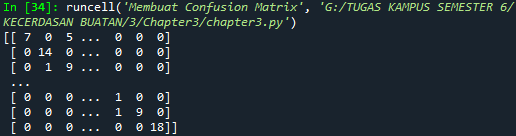
\includegraphics[scale=0.7]{figures/chapter3-5.png}}
              \centerline{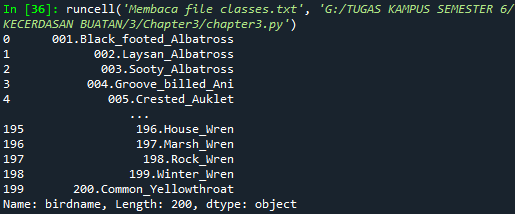
\includegraphics[scale=0.7]{figures/chapter3-5a.png}}
              \centerline{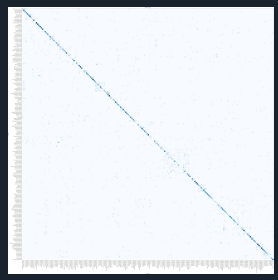
\includegraphics[scale=1.3]{figures/chapter3-5b.png}}
              \caption{Confusion Matrix - Chapter3}
              \label{Confusion Matrix - Chapter3}
          \end{figure}
          \newpage

    \item jalankan program klasifikasi SVM dan Decission Tree pada bagian teori bab ini. Tunjukkan keluarannya dari komputer sendiri dan artikan maksud setiap luaran yang didapatkan.
    \begin{figure}[ht]
        \centerline{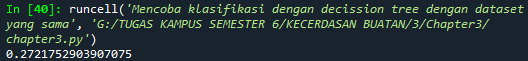
\includegraphics[scale=0.7]{figures/chapter3-6.png}}
        \centerline{\includegraphics[scale=0.7]{figures/chapter3-6a.png}}
        \caption{Klasifikasi SVM - Chapter3}
        \label{Klasifikasi SVM - Chapter3}
    \end{figure}

    \item jalankan program cross validaiton pada bagian teori bab ini. Tunjukkan keluarannya dari komputer sendiri dan artikan maksud setiap luaran yang didapatkan.
    \begin{figure}[ht]
        \centerline{\includegraphics[scale=0.7]{figures/chapter3-7.png}}
        \centerline{\includegraphics[scale=0.7]{figures/chapter3-7a.png}}
        \centerline{\includegraphics[scale=0.7]{figures/chapter3-7b.png}}
        \caption{Cross Validaiton - Chapter3}
        \label{Cross Validaiton - Chapter3}
    \end{figure}
    \newpage

    \item jalankan program pengamatan komponen informasi pada bagian teori bab ini. Tunjukkan keluarannya dari komputer sendiri dan artikan maksud setiap luaran yang didapatkan.
    \begin{figure}[ht]
        \centerline{\includegraphics[scale=0.7]{figures/chapter3-8.png}}
        \centerline{\includegraphics[scale=1.3]{figures/chapter3-8a.png}}
        \caption{Komponen Informasi - Chapter3}
        \label{Komponen Informasi - Chapter3}
    \end{figure}
\end{enumerate}


\section{Penanganan Error}
Dari percobaan yang dilakukan di atas, error yang kita dapatkan di dokumentasikan dan di selesaikan(nilai 5 per error yang ditangani. Untuk hari kedua):

\begin{enumerate}
    \item skrinsut error
    \item Tuliskan kode eror dan jenis errornya
    \item Solusi pemecahan masalah error tersebut
\end{enumerate}

\section{Presentasi Tugas}
Pada pertemuan ketiga ini, diadakan tiga penilaiain yaitu penilaian untuk tugas mingguan seperti sebelumnya dengan nilai maksimal 100. Kemudian dalam satu minggu kedepan maksimal sebelum waktu mata kuliah kecerdasan buatan. Ada presentasi tugas bab ini dan bab sebelumnya dengan nilai presentasi yang terpisah masing-masing 100. Jadi ada tiga komponen penilaiain pada pertemuan ini yaitu :
\begin{enumerate}
    \item tugas minggu hari ini dan besok (maks 100). pada chapter ini
    \item presentasi decission tree (maks 100). Mempraktekkan kode python dan menjelaskan cara kerjanya.
    \item presentasi Random Forest (maks 100).Mempraktekkan kode python dan menjelaskan cara kerjanya.
\end{enumerate}
Waktu presentasi pada jam kerja di IRC. Kriteria penilaian presentasi sangat sederhana, jika presenter tidak bisa menjawab pertanyaan asisten maka nilai nol. Jika semua pertanyaan bisa dijawab maka nilai 100. Presentasi bisa diulang apabila nilai nol sampai bisa mendapatkan nilai 100 dalam waktu satu minggu kedepan.



%\chapter{Klasifikasi Teks}

Untuk pratikum saati ini menggunakan buku \textit{Python Artificial Intelligence Projects for Beginners}\cite{eckroth2018python}. Dengan praktek menggunakan python 3 dan editor anaconda dan library python scikit-learn.
Kode program ada di https://github.com/PacktPublishing/Python-Artificial-Intelligence-Projects-for-Beginners .
Tujuan pembelajaran pada pertemuan pertama antara lain:
\begin{enumerate}
	\item
	      Mengerti implementasi klasifikasi pada teks
	\item
	      Mengerti teknik machine learning
	\item
	      Memahami Bag of Words
\end{enumerate}

Tugas dengan cara dikumpulkan dengan pull request ke github dengan menggunakan latex pada repo yang dibuat oleh asisten riset. Kode program menggunakan input listing ditaruh di folder src ekstensi .py dan dipanggil ke latex dengan input listings. Tulisan dan kode tidak boleh plagiat, menggunakan bahasa indonesia yang sesuai dengan gaya bahasa buku teks.

\section{Teori}
Menggunakan teknik bag-of-words pada klasifikasi berbasis text dan kata untuk mengklasifikasikan komentar yang ada di internet sebagai spam atau bukan. Atau bisa juga untuk melakukan identifikasi sebuah review apakah positive atau negatif.


\subsection{Vektorisasi data}
Pertama kita lakukan vektorisasi dari dataset. Lankah pertama kita baca terlebih dahulu dengan perintah \ref{lst:4.0}.
\begin{lstlisting}[caption=Membaca data file txt,label={lst:4.0}]
import pandas as pd
d = pd.read_csv("Youtube01-Psy.csv")
\end{lstlisting}

Memanggil library vektorisasi dari sci-kit lern, dengan menggunakan listing \ref{lst:4.1}.

\begin{lstlisting}[caption=Instansiasi Vektorizer,label={lst:4.1}]
from sklearn.feature_extraction.text import CountVectorizer
vectorizer = CountVectorizer()
\end{lstlisting}

Memilih kolom CONTENT dari dataframe d untuk di vektorisasi kemudian menampungnya pada variabel dvec menggunakan listing \ref{lst:4.2}.
\begin{lstlisting}[caption=Vektorisasi data dari atribut CONTENT,label={lst:4.2}]
dvec = vectorizer.fit_transform(d['CONTENT'])
dvec
\end{lstlisting}

Melihat daftar kata yang di vektorisasi. lalu kita simpan isinya pada variabel daptarkata dengan menggunakan perintah pada listing \ref{lst:4.3}.
\begin{lstlisting}[caption=Mendapatkan Daftar Kata,label={lst:4.3}]
daptarkata=vectorizer.get_feature_names()
\end{lstlisting}


Lakukan pengocokan data sehingga data terlihat random, perintahnya ada di listing \ref{lst:4.6}. Lalu kita cek kembali datanya pada variabel dshuf.
\begin{lstlisting}[caption=Mengocok Data Frame,label={lst:4.6}]
dshuf = d.sample(frac=1)
\end{lstlisting}

kemudian kita melakukan pemisahan antara data set untuk training dan test dengan perintah di listing \ref{lst:4.7}.
\begin{lstlisting}[caption=Memisahkan data frame,label={lst:4.7}]
d_train=dshuf[:300]
d_test=dshuf[300:]
\end{lstlisting}

Kita lakukan training perintah listing \ref{lst:4.8}.
\begin{lstlisting}[caption=Training pada vektorisasi atau yang disebut transform dan fit,label={lst:4.8}]
d_train_att=vectorizer.fit_transform(d_train['CONTENT'])
d_train_att
\end{lstlisting}

Lalu kita lakukan transformasi saja tanpa training pada data testing dengan perintah listing \ref{lst:4.9}.
\begin{lstlisting}[caption=Transform tanpa fit dari data testing,label={lst:4.9}]
d_test_att=vectorizer.transform(d_test['CONTENT'])
d_test_att
\end{lstlisting}

Pengambilan label klasifikasi spam dari kolom CLASS dengan perintah listing \ref{lst:4.10}.
\begin{lstlisting}[caption=Pengambilan label dari data testing dan training,label={lst:4.10}]
d_train_label=d_train['CLASS']
d_test_label=d_test['CLASS']
\end{lstlisting}



\subsection{Klasifikasi dengan Random Forest}
Setelah lakukan vektorisasi. Kita panggil kelas RandomForestClassifier. dengan n estimators sebanyak 80 yang artinya kita akan membuat 80 tree dengan tanpa batasan pengambilan atribut atau kolom dengan perintah listing \ref{lst:4.11}.
\begin{lstlisting}[caption=Instansiasi kelas Random Forest,label={lst:4.11}]
from sklearn.ensemble import RandomForestClassifier
clf=RandomForestClassifier(n_estimators=80)
\end{lstlisting}


Kemudian lakukan fit untuk membangun random forest yang sudah ditentukan dengan banyak tree sebanyak 80 dengan perintah listing \ref{lst:4.12}.
\begin{lstlisting}[caption=Fitting random forest dengan dataset training,label={lst:4.12}]
clf.fit(d_train_att,d_train_label)
\end{lstlisting}


Hasilnya bisa kita lakukan prediksi dari data testing dengan perintah listing \ref{lst:4.13}.
\begin{lstlisting}[caption=Melihat Hasil prediksi,label={lst:4.13}]
clf.predict(d_test_att)
\end{lstlisting}

Untuk besaran skornya dengan perintah listing \ref{lst:4.14}
\begin{lstlisting}[caption=Score perolehan dari klasifikasi,label={lst:4.14}]
clf.score(d_test_att,d_test_label)
\end{lstlisting}

\subsection{Confusion Matrix}
Dari RF kita coba petakan ke dalam Confusion Matrix dan lihat hasilnya dengan perintah listing \ref{lst:4.15}.
\begin{lstlisting}[caption=Membuat Confusion Matrix,label={lst:4.15}]
from sklearn.metrics import confusion_matrix
pred_labels = clf.predict(d_test_att)
cm=confusion_matrix(d_test_label, pred_labels)
\end{lstlisting}



\subsection{Pengecekan Cross Validation}
Pengeceken Cross Validation untuk random forest dengan perintah \ref{lst:4.21}.
\begin{lstlisting}[caption=Hasil Cross Validation random forest,label={lst:4.21}]
from sklearn.model_selection import cross_val_score
scores = cross_val_score(clf,d_train_att,d_train_label,cv=5)

skorrata2=scores.mean()
skoresd=scores.std()
\end{lstlisting}


\section{Soal Teori}
Praktek teori penunjang yang dikerjakan(nilai 5 per nomor, untuk hari pertama) :
\begin{enumerate}
	\item
	      Jelaskan apa itu klasifikasi teks, sertakan gambar ilustrasi buatan sendiri.
	\item
	      Jelaskan mengapa klasifikasi bunga tidak bisa menggunakan machine learning, sertakan ilustrasi sendiri.
	\item
	      Jelaskan bagaimana teknik pembelajaran mesin pada teks pada kata-kata yang digunakan di youtube,jelaskan arti per atribut data csv dan sertakan ilustrasi buatan sendiri.
	\item
	      Jelaskan apa yang dimaksud vektorisasi data.
	\item
	      Jelaskan apa itu bag of words dengan kata-kata yang sederhana dan ilustrasi sendiri.
	\item
	      Jelaskan apa itu TF-IDF, ilustrasikan dengan gambar sendiri.
\end{enumerate}



\section{Praktek Program}
Tugas anda adalah,praktekkan dan jelaskan dengan menggunakan bahasa yang mudah dimengerti dan bebas plagiat dan wajib skrinsut dari komputer sendiri masing masing nomor di bawah ini(nilai 5 masing masing pada hari kedua).

\begin{enumerate}
	\item buat aplikasi sederhana menggunakan pandas, buat data dummy format csv sebanyak 500 baris dan melakukan load ke dataframe panda.jelaskan arti setiap baris kode yang dibuat(harus beda dengan teman sekelas)
	      \begin{figure}[ht]
		      \centerline{\includegraphics[scale=0.7]{figures/chappter4-1.png}}
		      \caption{Aplikasi Pandas - Chapter4}
		      \label{Aplikasi Pandas - Chapter4}
	      \end{figure}
	      \newpage

	\item dari dataframe tersebut dipecah menjadi dua dataframe yaitu 450 row pertama dan 50 row sisanya(harus beda dengan teman sekelas)
	      \begin{figure}[ht]
		      \centerline{\includegraphics[scale=0.7]{figures/chappter4-2.png}}
		      \caption{Dataframe dipecah menjadi dua - Chapter4}
		      \label{Dataframe dipecah menjadi dua- Chapter4}
	      \end{figure}
	      \newpage

	\item pratekkan vektorisasi dan klasifikasi dari data (NPM mod 4, jika 0 maka katty perry, 1 LMFAO, 2 Eminem, 3 Shakira) dengan Decission Tree. Tunjukkan keluarannya dari komputer sendiri dan artikan maksud setiap luaran yang didapatkan.
	      \begin{figure}[ht]
		      \centerline{\includegraphics[scale=0.7]{figures/chappter4-3.png}}
		      \caption{Vektorisasi dan Klasifikasi 1194018 = mod 2 - Chapter4}
		      \label{Vektorisasi dan Klasifikasi 1194018 = mod 2 - Chapter4}
	      \end{figure}

	\item Cobalah klasifikasikan dari data vektorisasi yang di tentukan di nomor sebelumnya dengan klasifikasi SVM. Tunjukkan keluarannya dari komputer sendiri dan artikan maksud setiap luaran yang didapatkan.
	      \begin{figure}[ht]
		      \centerline{\includegraphics[scale=0.7]{figures/chappter4-4.png}}
		      \centerline{\includegraphics[scale=0.7]{figures/chappter4-4a.png}}
	      \end{figure}
	      \newpage
	      \begin{figure}[ht]
		      \centerline{\includegraphics[scale=0.7]{figures/chappter4-4b.png}}
		      \centerline{\includegraphics[scale=0.7]{figures/chappter4-4c.png}}
		      \centerline{\includegraphics[scale=0.7]{figures/chappter4-4d.png}}
	      \end{figure}
	      \newpage
	      \begin{figure}[ht]
		      \centerline{\includegraphics[scale=0.7]{figures/chappter4-4e.png}}
		      \centerline{\includegraphics[scale=0.7]{figures/chappter4-4f.png}}
		      \caption{Vektorisasi dan Klasifikasi - Chapter4}
		      \label{Vektorisasi dan Klasifikasi- Chapter4}
	      \end{figure}

	\item Cobalah klasifikasikan dari data vektorisasi yang di tentukan di nomor sebelumnya dengan klasifikasi Decission Tree. Tunjukkan keluarannya dari komputer sendiri dan artikan maksud setiap luaran yang didapatkan.
	      \begin{figure}[ht]
		      \centerline{\includegraphics[scale=0.7]{figures/chappter4-5.png}}
		      \caption{Vektorisasi dan Klasifikasi Decission Tree - Chapter4}
		      \label{Vektorisasi dan Klasifikasi Decission Tree - Chapter4}
	      \end{figure}

	\item Plotlah confusion matrix dari praktek modul ini menggunakan matplotlib.Tunjukkan keluarannya dari komputer sendiri dan artikan maksud setiap luaran yang didapatkan.
	      \begin{figure}[ht]
		      \centerline{\includegraphics[scale=0.7]{figures/chappter4-6.png}}
		      \caption{Confusion Matrix - Chapter4}
		      \label{Confusion Matrix - Chapter4}
	      \end{figure}

	\item jalankan program cross validaiton pada bagian teori bab ini. Tunjukkan keluarannya dari komputer sendiri dan artikan maksud setiap luaran yang didapatkan.
	\newpage
	\begin{figure}[ht]
		\centerline{\includegraphics[scale=0.7]{figures/chappter4-7.png}}
		\centerline{\includegraphics[scale=0.7]{figures/chappter4-7a.png}}
		\centerline{\includegraphics[scale=0.7]{figures/chappter4-7b.png}}
		\centerline{\includegraphics[scale=0.7]{figures/chappter4-7c.png}}
		\caption{Cross Validaiton - Chapter4}
		\label{Cross Validaiton - Chapter4}
	\end{figure}

	\item Buatlah program pengamatan komponen informasi pada bagian teori bab ini. Tunjukkan keluarannya dari komputer sendiri dan artikan maksud setiap luaran yang didapatkan.
	\begin{figure}[ht]
		\centerline{\includegraphics[scale=0.7]{figures/chappter4-8.png}}
		\centerline{\includegraphics[scale=0.7]{figures/chappter4-8a.png}}
		\caption{Komponen Informasi - Chapter4}
		\label{Komponen Informasi - Chapter4}
	\end{figure}
\end{enumerate}


\section{Penanganan Error}
Dari praktek pemrograman yang dilakukan di modul ini, error yang kita dapatkan(hasil komputer sendiri) di dokumentasikan dan di selesaikan(nilai 5 per error yang ditangani. Untuk hari kedua):

\begin{enumerate}
	\item skrinsut error
	\item Tuliskan kode eror dan jenis errornya
	\item Solusi pemecahan masalah error tersebut
\end{enumerate}

\section{Presentasi Tugas}
Pada pertemuan ketiga ini, diadakan tiga penilaiain yaitu penilaian untuk tugas mingguan seperti sebelumnya dengan nilai maksimal 100. Kemudian dalam satu minggu kedepan maksimal sebelum waktu mata kuliah kecerdasan buatan. Ada presentasi kematerian dengan nilai presentasi yang terpisah masing-masing 100. Jadi ada tiga komponen penilaiain pada pertemuan ini yaitu :
\begin{enumerate}
	\item tugas minggu hari ini dan besok (maks 100). pada chapter ini
	\item presentasi Vektorisasi (maks 100). Mempraktekkan kode python dan menjelaskan cara kerjanya.
	\item presentasi cara kerja Data Frame di Pandas (maks 100).Mempraktekkan kode python dan menjelaskan cara kerjanya.
\end{enumerate}
Waktu presentasi pada jam kerja di IRC. Kriteria penilaian presentasi sangat sederhana, presenter akan ditanyai 20 pertanyaan tentang pemahamannya menggunakan python untuk kecerdasan buatan. jika presenter tidak bisa menjawab satu pertanyaan asisten maka nilai nol. Jika semua pertanyaan bisa dijawab maka nilai 100. Presentasi bisa diulang apabila gagal, sampai bisa mendapatkan nilai 100 dalam waktu satu minggu kedepan.



%\include{section/chapter5}
%\include{section/chapter6}
%\include{section/chapter7}
%\include{section/chapter8}
%\include{section/chapter9}
%\include{section/chapter10}
%\include{section/chapter11}
%\include{section/chapter12}
%\include{section/chapter13}
%\include{section/chapter14}

%now enable appendix numbering format and include any appendices
%\appendix
%\include{section/appendix1}
%\include{section/appendix2}

%next line adds the Bibliography to the contents page
%\addcontentsline{toc}{chapter}{Bibliography}
%uncomment next line to change bibliography name to references
%\renewcommand{\bibname}{References}
%\bibliography{references}        %use a bibtex bibliography file refs.bib
%\bibliographystyle{plain}  %use the plain bibliography style

\end{document}

